\documentclass[a4paper,12pt]{report}

\usepackage{alltt, fancyvrb, url}
\usepackage{graphicx}
\usepackage[utf8]{inputenc}
\usepackage{float}
\usepackage{xcolor}
\usepackage{hyperref}

% Questo commentalo se vuoi scrivere in inglese.
\usepackage[italian]{babel}

\usepackage[italian]{cleveref}

\title{Meta-relazione per\\``Programmazione ad Oggetti''}

\author{Filippo Greppi, Elena Fucci, Spaccini Ettore}
\date{\today}


\begin{document}

\maketitle

\begin{abstract}
 %%

\end{abstract}

\tableofcontents

\chapter{Analisi}

\section{Descrizione e requisiti}
Il software mira allo sviluppo del videogioco “Mind-Escape”, un’avventura psicologica e di suspense. Il giocatore assume il ruolo di un personaggio che si sveglia in una stanza sconosciuta, senza memoria di come ci sia arrivato. L’obiettivo del gioco è fuggire da questa prigionia, risolvendo una serie di enigmi che si presentano in diverse stanze. Ogni enigma risolto porta il giocatore più vicino alla vittoria, aprendo la via verso la stanza successiva.
%
Per avanzare, il giocatore deve raccogliere e utilizzare vari oggetti, che vengono gestiti attraverso un inventario. Questi oggetti sono essenziali per risolvere enigmi e accedere a nuove stanze.
%
La partita si concluderà quando il giocatore raggiungerà e risolverà l’enigma finale, riuscendo a fuggire dall’ultima stanza.
%

\subsubsection{Requisiti funzionali}
\begin{itemize}
	\item Il personaggio deve poter muoversi nella mappa, gestendo le collisioni con ostacoli e pareti
	\item Il gioco deve permettere al personaggio di interagire con gli oggetti nelle stanze (es. raccogliere, esaminare, usare).
	\item Il personaggio deve disporre di un inventario che permetta di gestire gli oggetti raccolti.
	\item Il sistema deve verificare automaticamente la correttezza delle soluzioni degli enigmi.
\end{itemize}

\subsubsection{Requisiti non funzionali}
\begin{itemize}
	\item Salvataggio dello stato della partita
	\item Deve essere garantita una modularità del codice per consentire l'aggiunta futura di nuove stanze o enigmi.
	\item Ridimensionabilità della finestra di gioco
\end{itemize}

\section{Modello del Dominio}

Mind Escape è un gioco ambientato in un mondo suddiviso in più stanze, attraverso le quali il giocatore può muoversi ed interagire con vari oggetti. 
L’avventura ha inizio in una stanza iniziale, da cui il giocatore potrà accedere progressivamente alle altre stanze. 
Il passaggio tra le stanze avviene mediante porte, che possono essere sbloccate risolvendo enigmi o utilizzando oggetti raccolti durante il gioco. L'obiettivo finale è raggiungere l’ultima stanza e interagire con uno specifico oggetto, evento che determina la vittoria.

\begin{figure}[h]  % [h] indica che la figura sarà posizionata il più vicino possibile
    \centering
    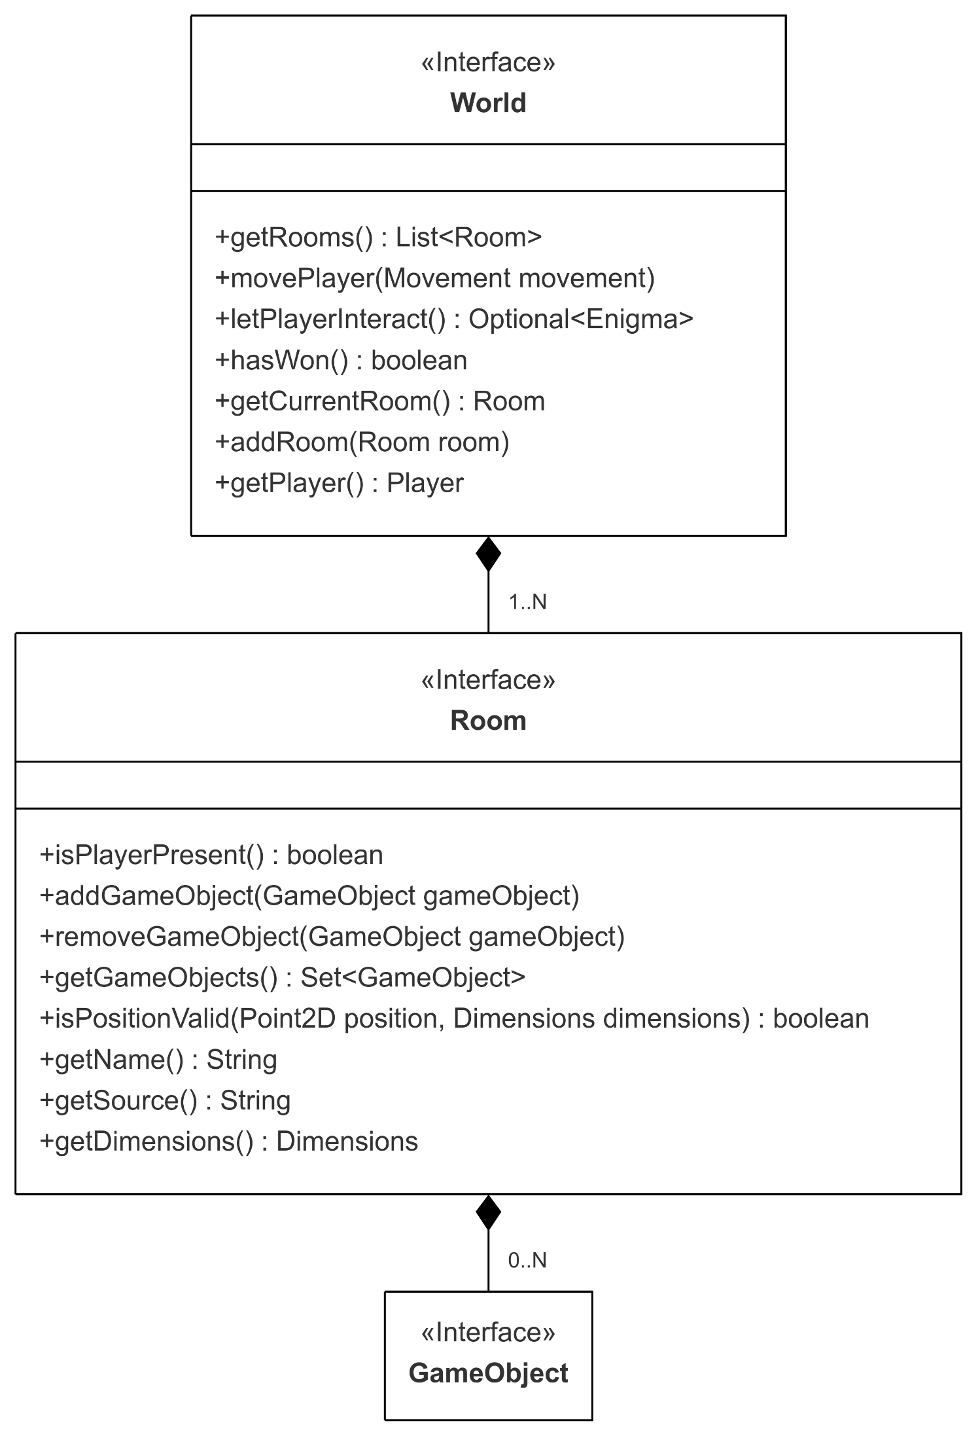
\includegraphics[width=0.8\textwidth]{img/model.png}  % Modifica width se serve
    \caption{Esempio di game object}
    \label{img:gameObject}
\end{figure}

All'interno di ogni stanza possono essere presenti oggetti di gioco (GameObject), con i quali il giocatore può collidere. 
Gli oggetti di gioco si suddividono in due categorie principali:
\begin{itemize}
	\item Oggetti interagibili (Interactable): si distinguono in due sottocategorie:
	\begin{itemize}
		\item Oggetti raccoglibili (Pickable): possono essere raccolti dal giocatore ed inseriti nell’inventario, dove potranno essere utilizzati successivamente.
		\item Oggetti non raccoglibili (Unpickable): non possono essere raccolti, ma possono essere sbloccati tramite determinate azioni. Alcuni di essi possono essere associati alla risoluzione di un enigma.
	\end{itemize}
	L'interazione tra il giocatore e un oggetto interagibile può avvenire esclusivamente a seguito di una collisione. In seguito all'interazione, l'oggetto esegue un'azione predefinita che determina il suo comportamento e le conseguenze dell'interazione.
	\item Oggetti non interagibili (NonInteractable): questi oggetti hanno una funzione puramente estetica o di ambientazione, e non influenzano direttamente il gameplay. Tuttavia, il giocatore può collidere con essi.
\end{itemize}

\begin{figure}[h]  % [h] indica che la figura sarà posizionata il più vicino possibile
    \centering
    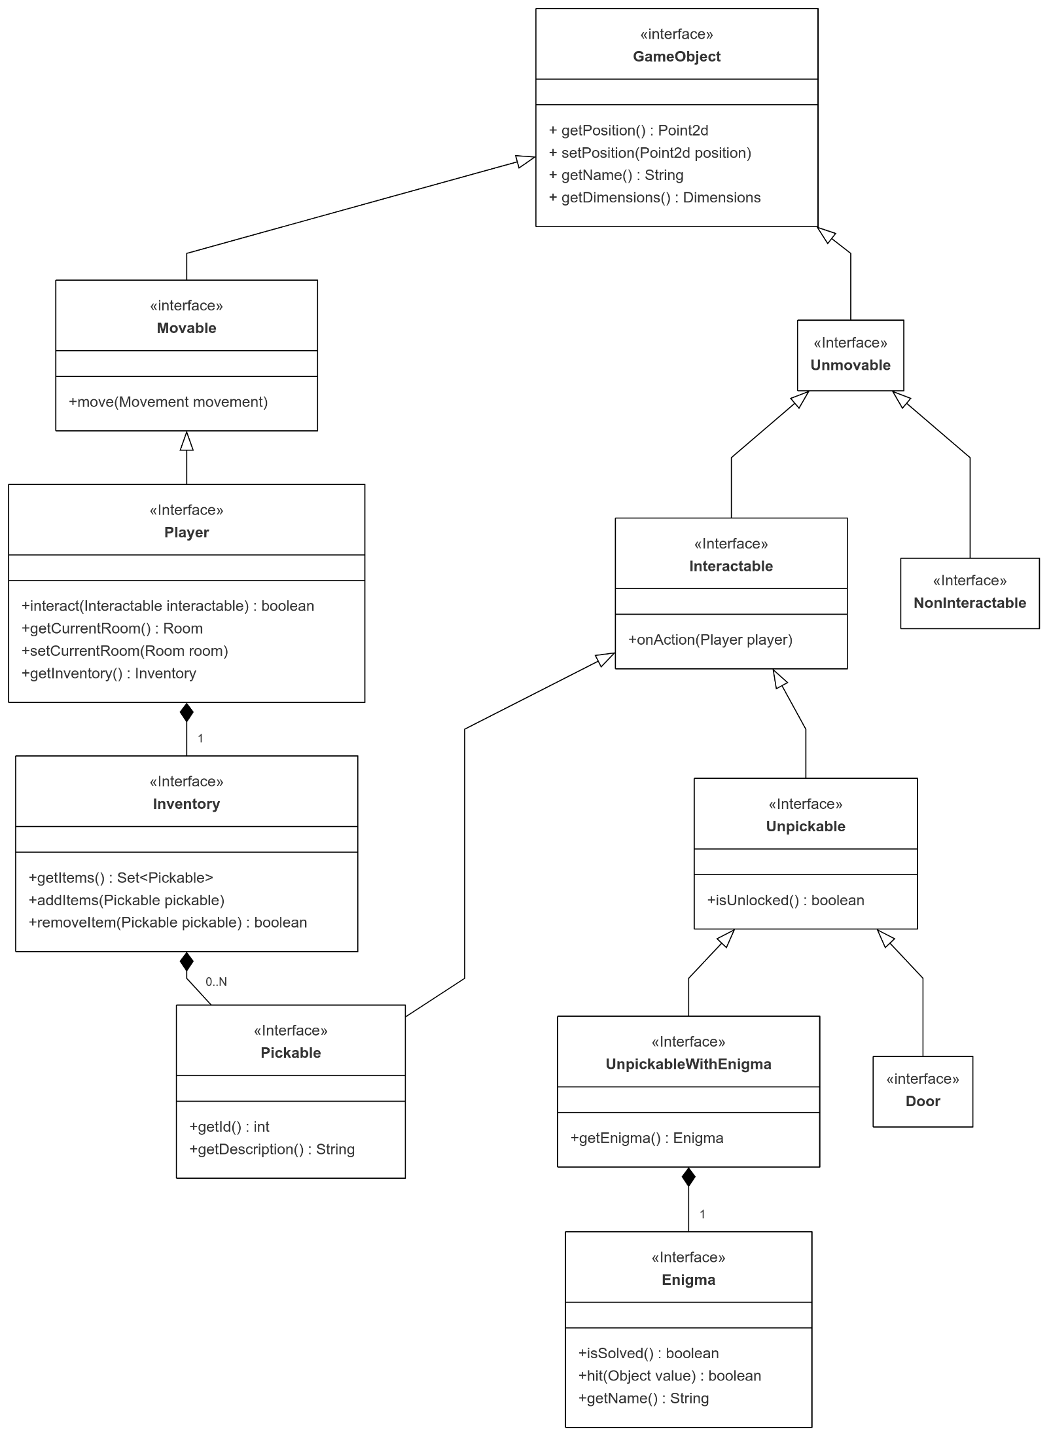
\includegraphics[width=0.8\textwidth]{img/gameObject.png}  % Modifica width se serve
    \caption{Esempio di game object}
    \label{img:gameObject}
\end{figure}
 % 
\chapter{Design}
\section{Architettura}
L'architettura di Mind-Escape segue il pattern architetturale MVC (Model-View-Controller), ma si compone di più strutture MVC modulari. 
Il sistema implementa un'interfaccia chiamata MainController, che ha il compito di cercare e attivare i controller appropriati in base alle azioni dell'utente. 
I controller disponibili sono quelli associati ai vari MVC, e sono suddivisi in due categorie principali:
\begin{itemize}
	\item LoopController: Gestisce gli MVC che richiedono un aggiornamento costante sia dal punto di vista logico che grafico. L'esecuzione di questi aggiornamenti può essere avviata o interrotta in base alle decisioni del MainController.
	\item 2.	ClickableController: Gestisce gli MVC che necessitano di un aggiornamento sia logico che grafico, ma solo in seguito a un'interazione esplicita dell'utente, come l'uso del mouse o la tastiera.
\end{itemize}
%
Ogni controller è in grado di notificare il MainController riguardo al passaggio al controller successivo. Il MainController è responsabile della creazione e gestione dei controller necessari, ottimizzando l'uso della memoria in base alle esigenze specifiche. 
Questo approccio consente di aggiungere un numero arbitrario di controller senza compromettere la struttura dell'applicazione.
%
Inoltre, Mind-Escape supporta la registrazione di input e output all'interno delle view di ciascun MVC.
Gli input rappresentano nuove informazioni inviate ai controller, che possono includere comandi da mouse, tastiera, o l'inserimento di password. 
Questi input sono generati dall'utente e possono scatenare eventi che modificano il controller corrente. Una volta ricevuti gli input, il MainController aggiorna la view corretta in output, permettendo un'interazione dinamica e fluida.
%
In sintesi, l'aggiunta di nuovi Model, Controller e View non richiede modifiche alla struttura centrale dell'applicazione, garantendo così una scalabilità e una modularità efficaci.
%

\begin{figure}[h]  % [h] indica che la figura sarà posizionata il più vicino possibile
    \centering
    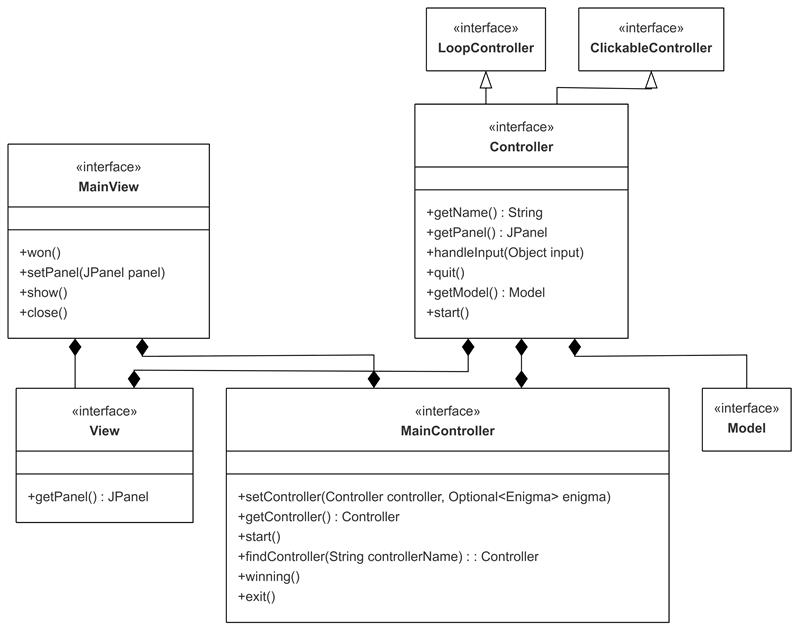
\includegraphics[width=0.8\textwidth]{img/mvc.png}  % Modifica width se serve
    \label{img:mvc}
\end{figure}

% arrivato qui
\section{Design dettagliato}
%% forse va messo la descrizione
\subsection{Elena Fucci}
%
\paragraph{Problema}Nel gioco Mind-Escape, quando un giocatore raccoglie degli oggetti, questi devono essere visualizzati all'interno di un inventario, che deve poter essere modificato durante il gioco.
La sfida è quella di garantire che l'inventario possa essere aggiornato dinamicamente e salvato in modo persistente, affinchè le modifiche possano essere recuperate anche in sessioni di gioco future. %%descrizione del problema
\paragraph{Soluzione}Il problema viene gestito tramite la creazione di un’interfaccia Player che si compone di un’interfaccia Inventory. 
L'inventario può essere aggiornato in tempo reale quando il giocatore raccoglie oggetti. 
Inoltre, il Player è direttamente collegato al mondo collegato a sua volta ad un file di salvataggio, il che consente di salvare lo stato corrente del giocatore, compreso l'inventario, su un file. 
In questo modo, il gioco è in grado di mantenere le modifiche correnti all'inventario e ripristinarle quando il giocatore riprende la partita. %% descrizione della soluzione
%
\begin{figure}[h]  % [h] indica che la figura sarà posizionata il più vicino possibile
    \centering
    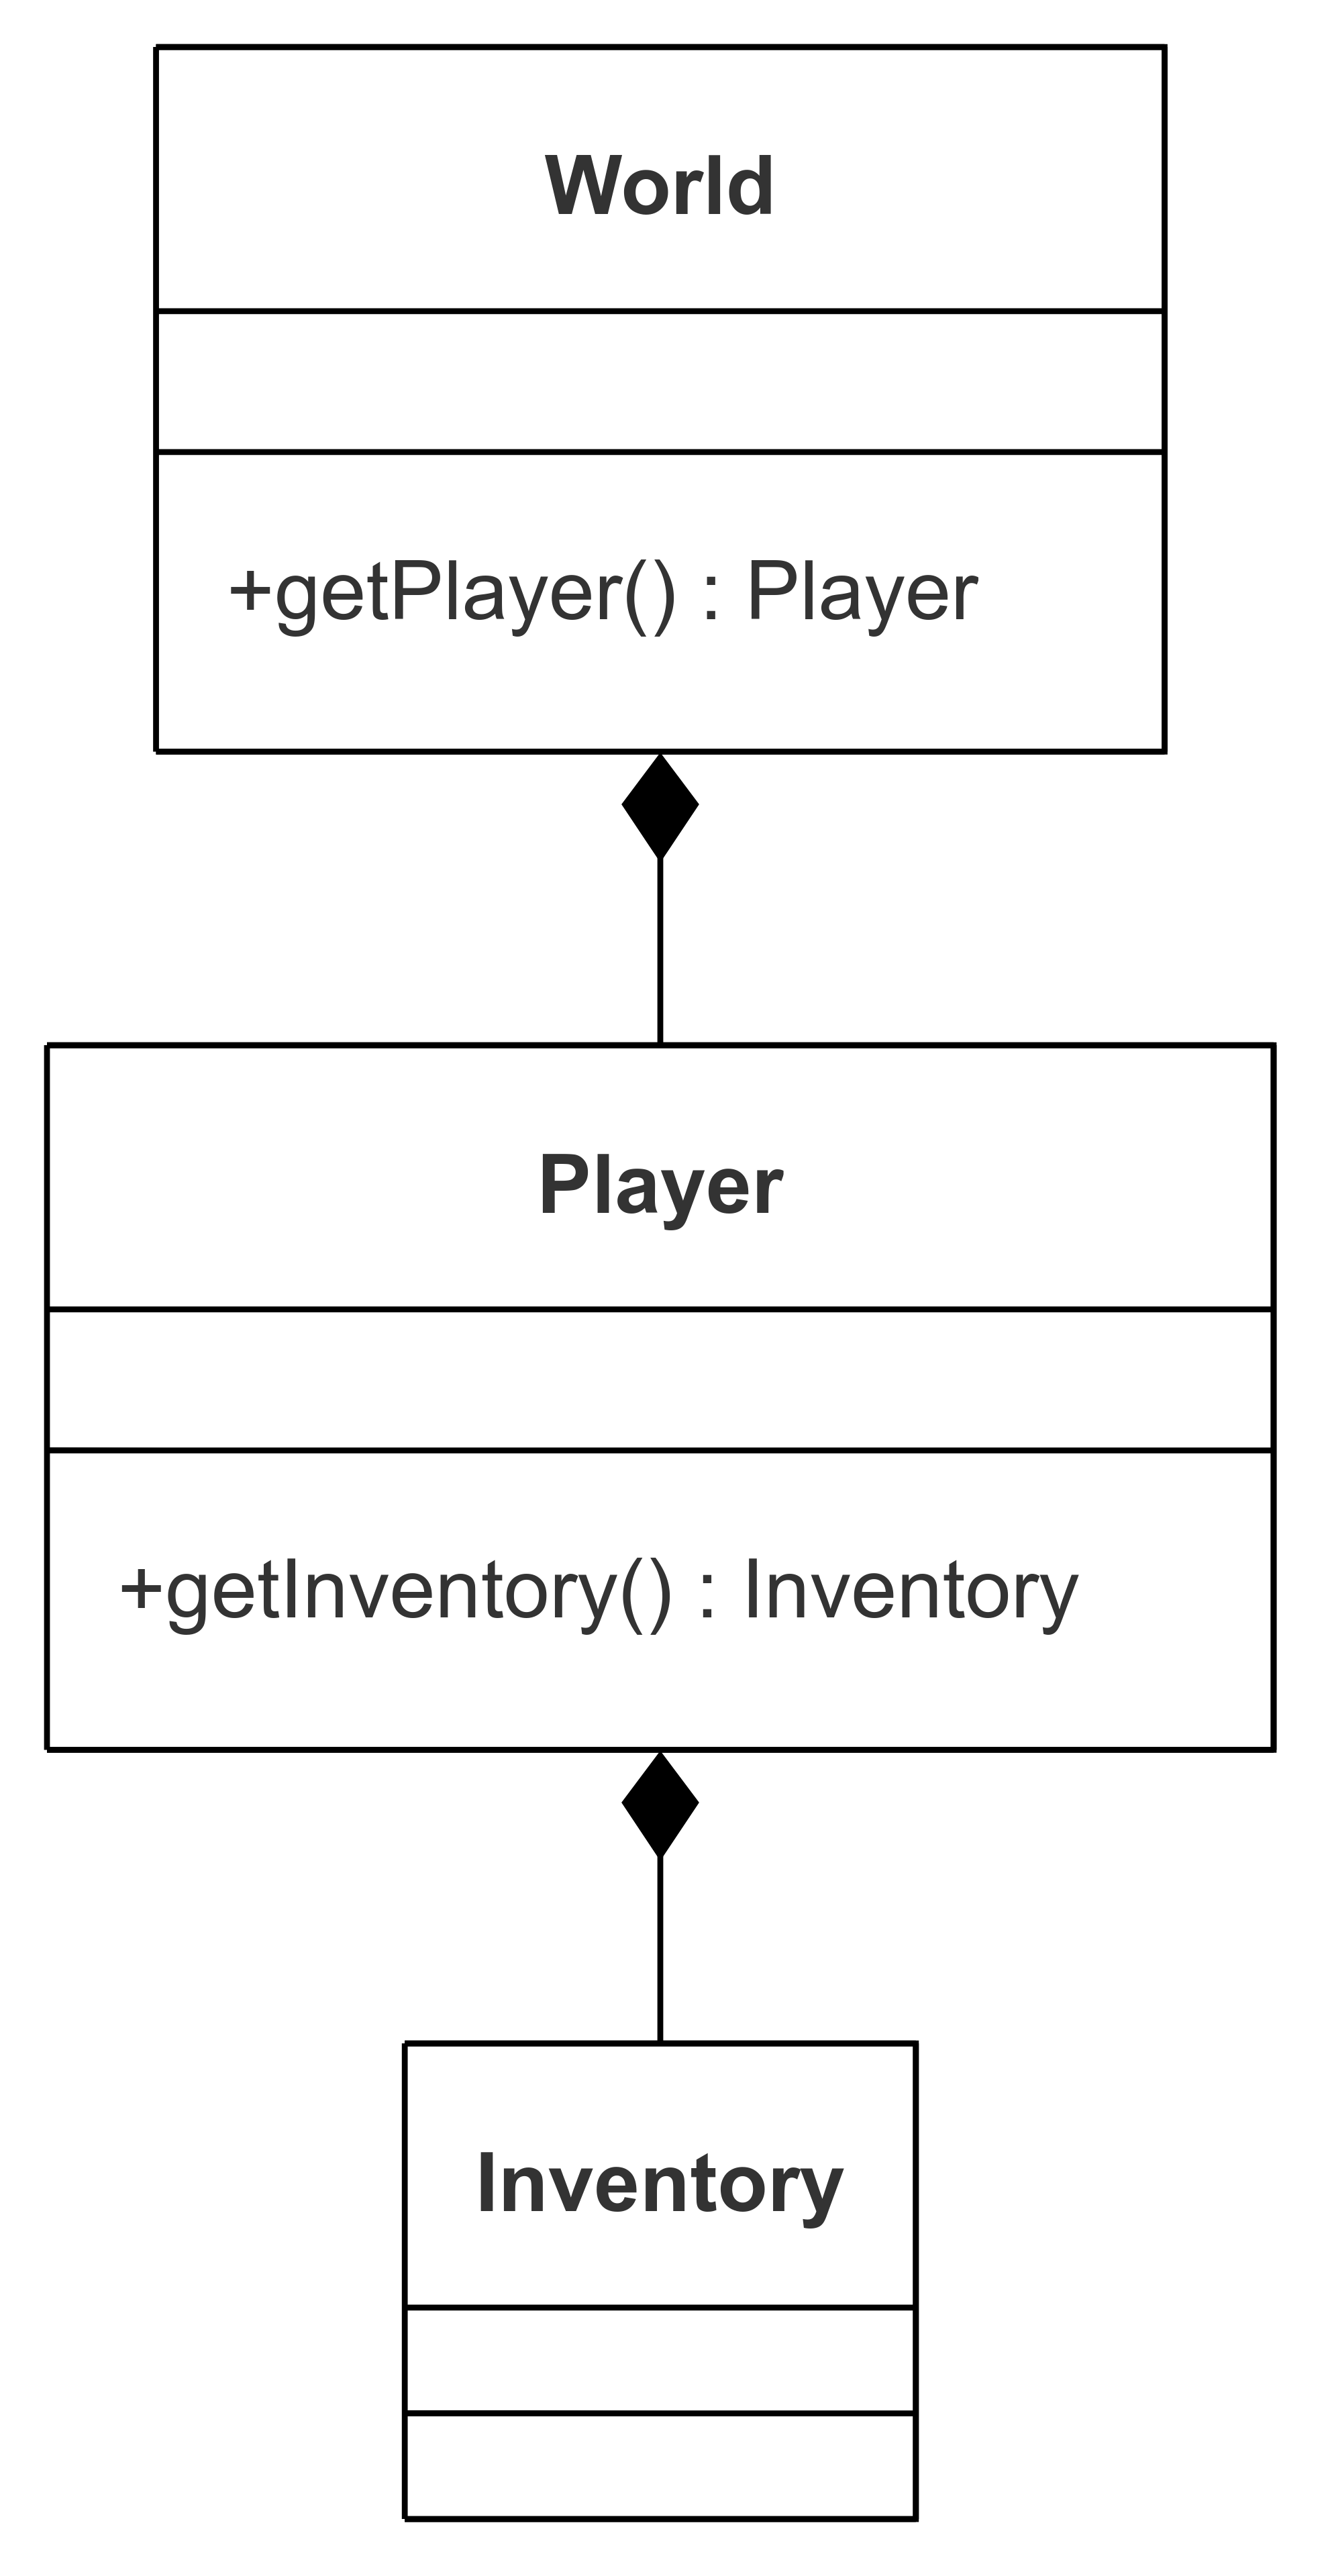
\includegraphics[width=0.8\textwidth]{img/player.png}  % Modifica width se serve
    \label{img:gameObject}
\end{figure}
%
\paragraph{Problema}All’interno del gioco sono presenti vari enigmi. Uno degli enigmi da risolvere è un puzzle. 
Per implementare questa parte, è necessario permettere al gioco di passare da una vista principale a una vista dedicata al puzzle, in modo che il giocatore possa interagire con il puzzle senza interruzioni. 
%
\paragraph{Soluzione}Per risolvere questo problema, ho adottato il pattern MVC (Model-View-Controller). 
Questo approccio consente al mainController di trasferire temporaneamente il controllo al controller dell’enigma, che si occupa di gestire la logica del puzzle e di visualizzare la vista del puzzle corrispondente. 
L’uso del pattern consente di separare chiaramente la logica del gioco dalla parte di view rendendo il codice più modulare. 
Poichè modifiche alla logica del puzzle non influenzano la vista, e viceversa, il che facilita l'aggiornamento o l'aggiunta di nuove funzionalità.
\begin{figure}[h]  % [h] indica che la figura sarà posizionata il più vicino possibile
    \centering
    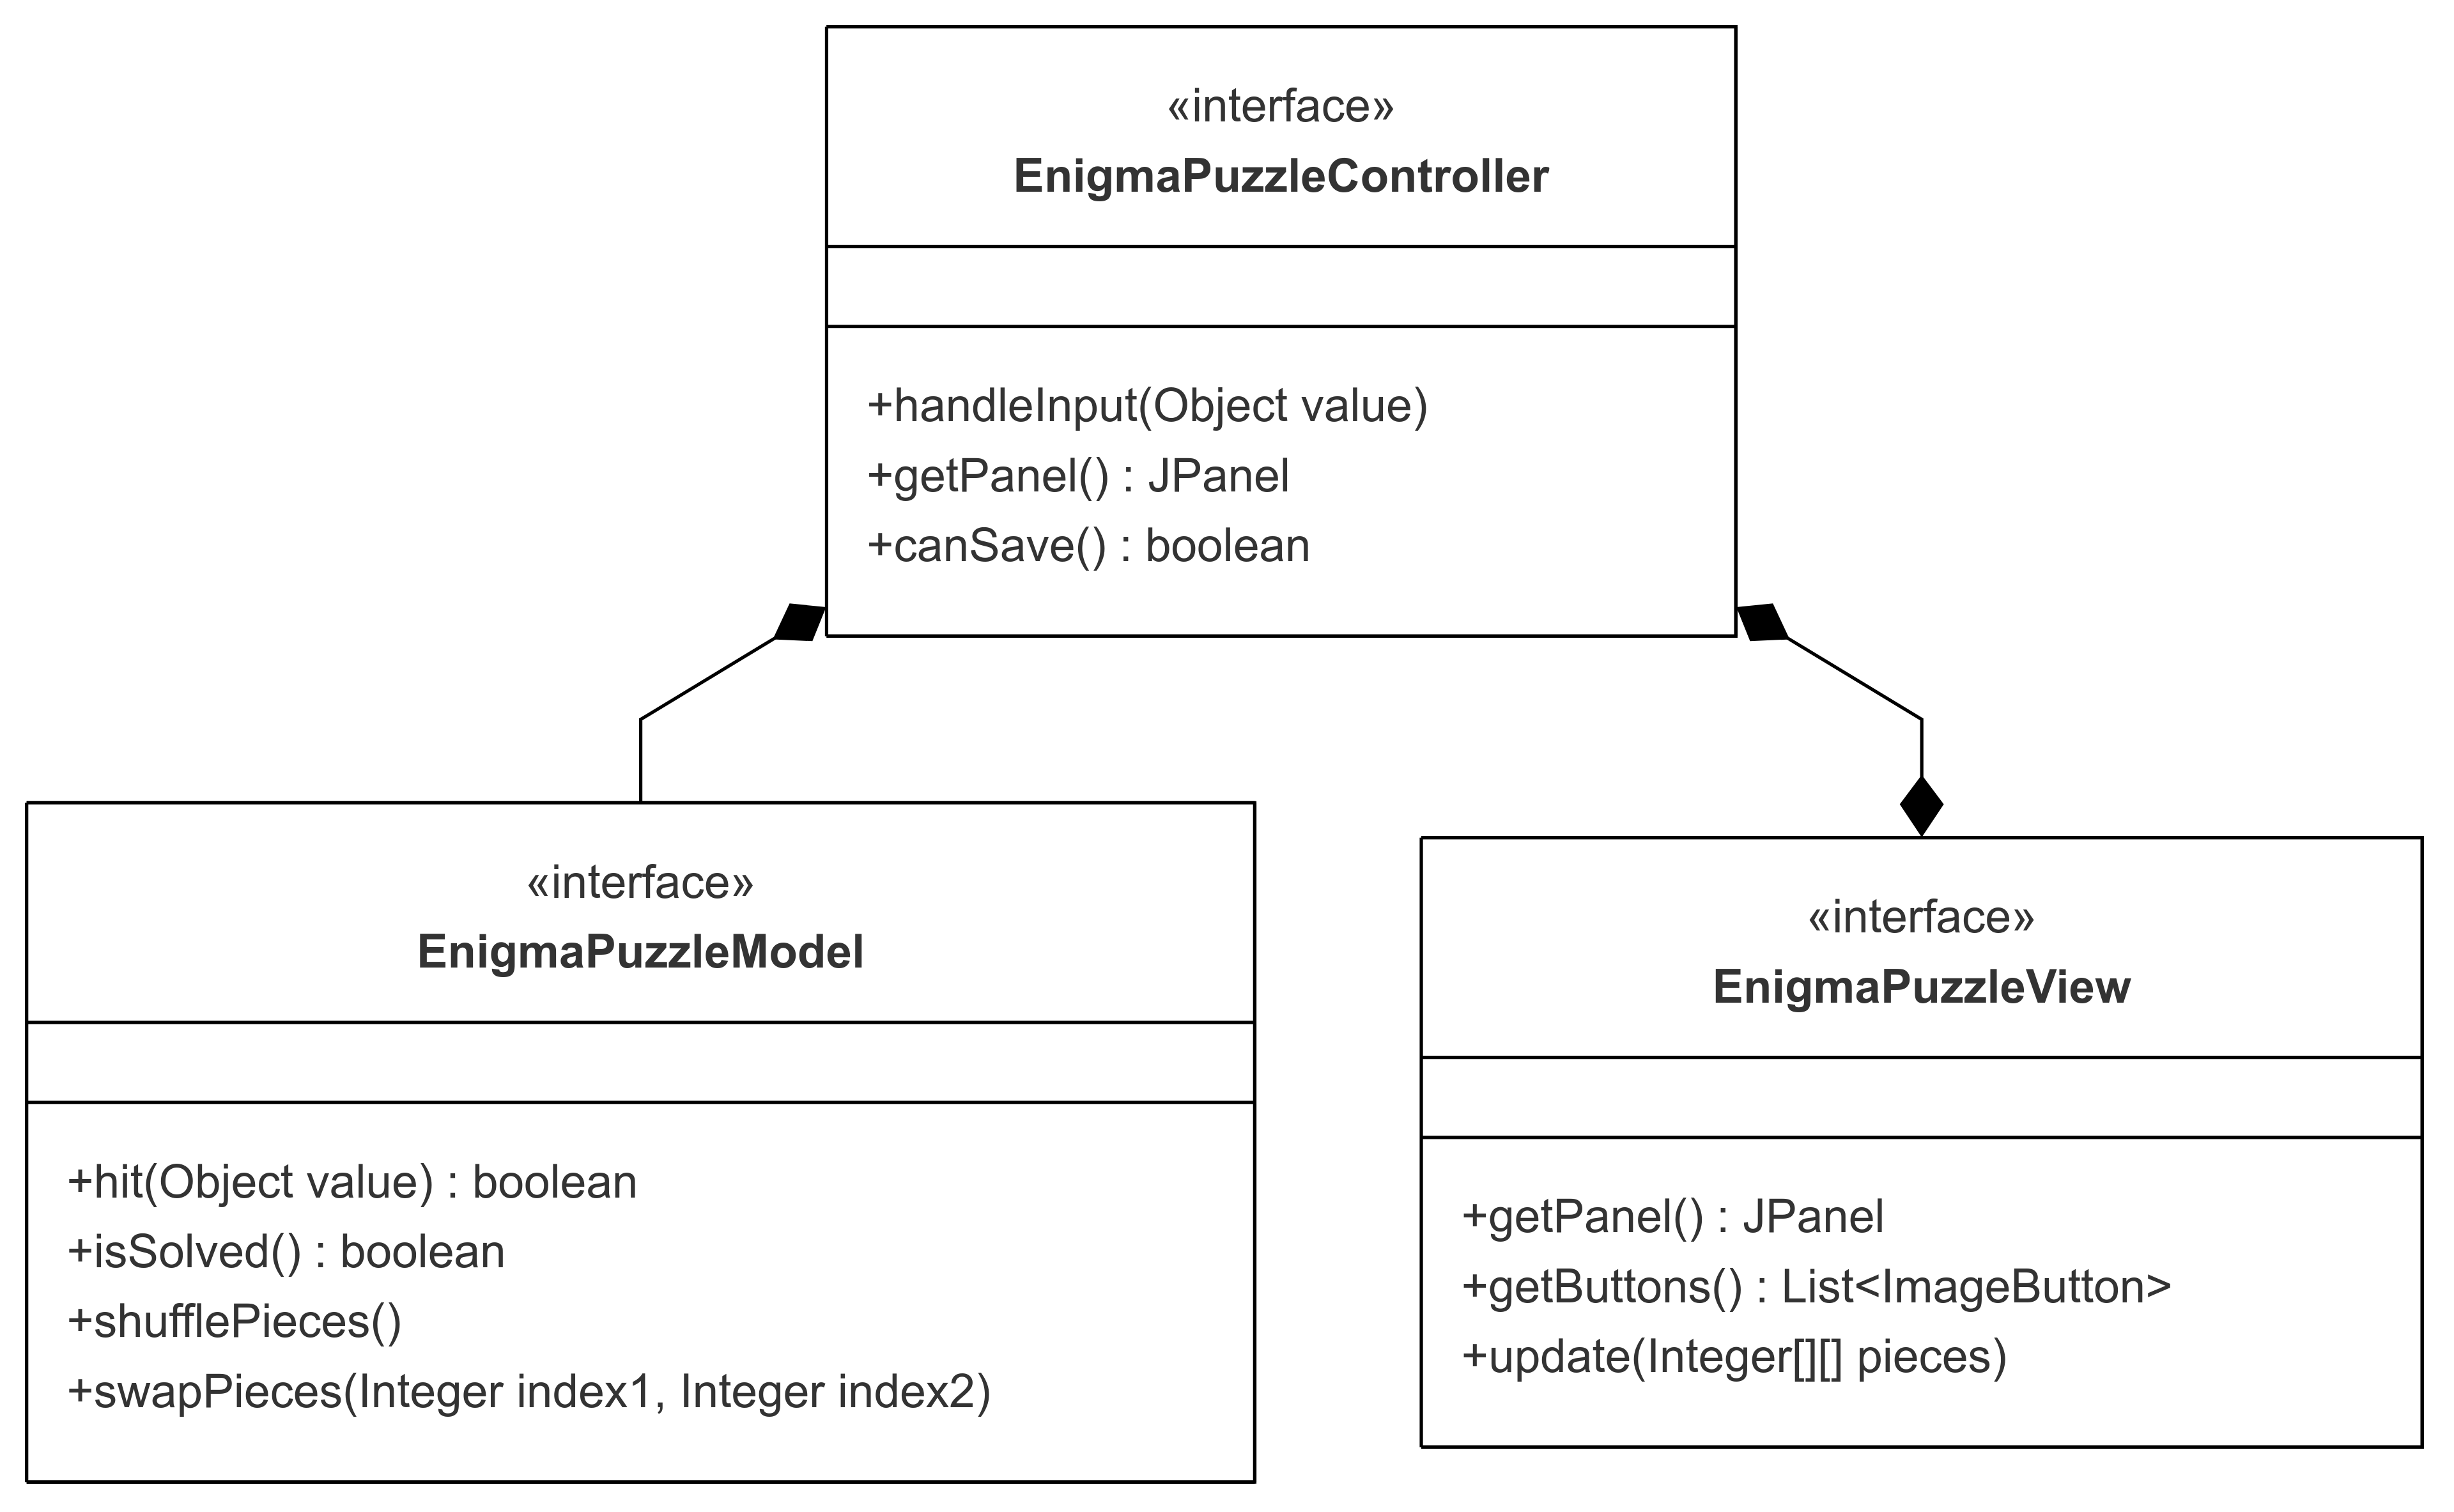
\includegraphics[width=0.8\textwidth]{img/puzzle.png}  % Modifica width se serve
    \label{img:gameObject}
\end{figure}
%
\paragraph{Problema}Nel gioco, l'inventario è utilizzato per visualizzare gli oggetti raccolti e alcuni indizi. La gestione dell'inventario deve permettere una visualizzazione chiara e aggiornata durante il gioco. Questo richiede una separazione della logica di gestione degli oggetti e dei dati dalla loro visualizzazione, al fine di garantire una gestione efficiente e flessibile dell'inventario.
%
\paragraph{Soluzione}Per risolvere il problema, è stato adottato il pattern MVC (Model-View-Controller). In questo schema, la logica di gestione dell'inventario è separata dalla sua visualizzazione, permettendo una chiara distinzione tra i dati (modello), l'interfaccia utente (vista) e il controllo (controller). Questa separazione consente di isolare le modifiche in una singola componente senza influire sulle altre.Poiché ogni componente ha un ruolo chiaro e definito, è più facile mantenere e aggiornare il codice, aggiungere nuove funzionalità o migliorare quelle esistenti diventa più semplice senza rischio di causare conflitti tra le diverse logiche.
\begin{figure}[h]  % [h] indica che la figura sarà posizionata il più vicino possibile
    \centering
    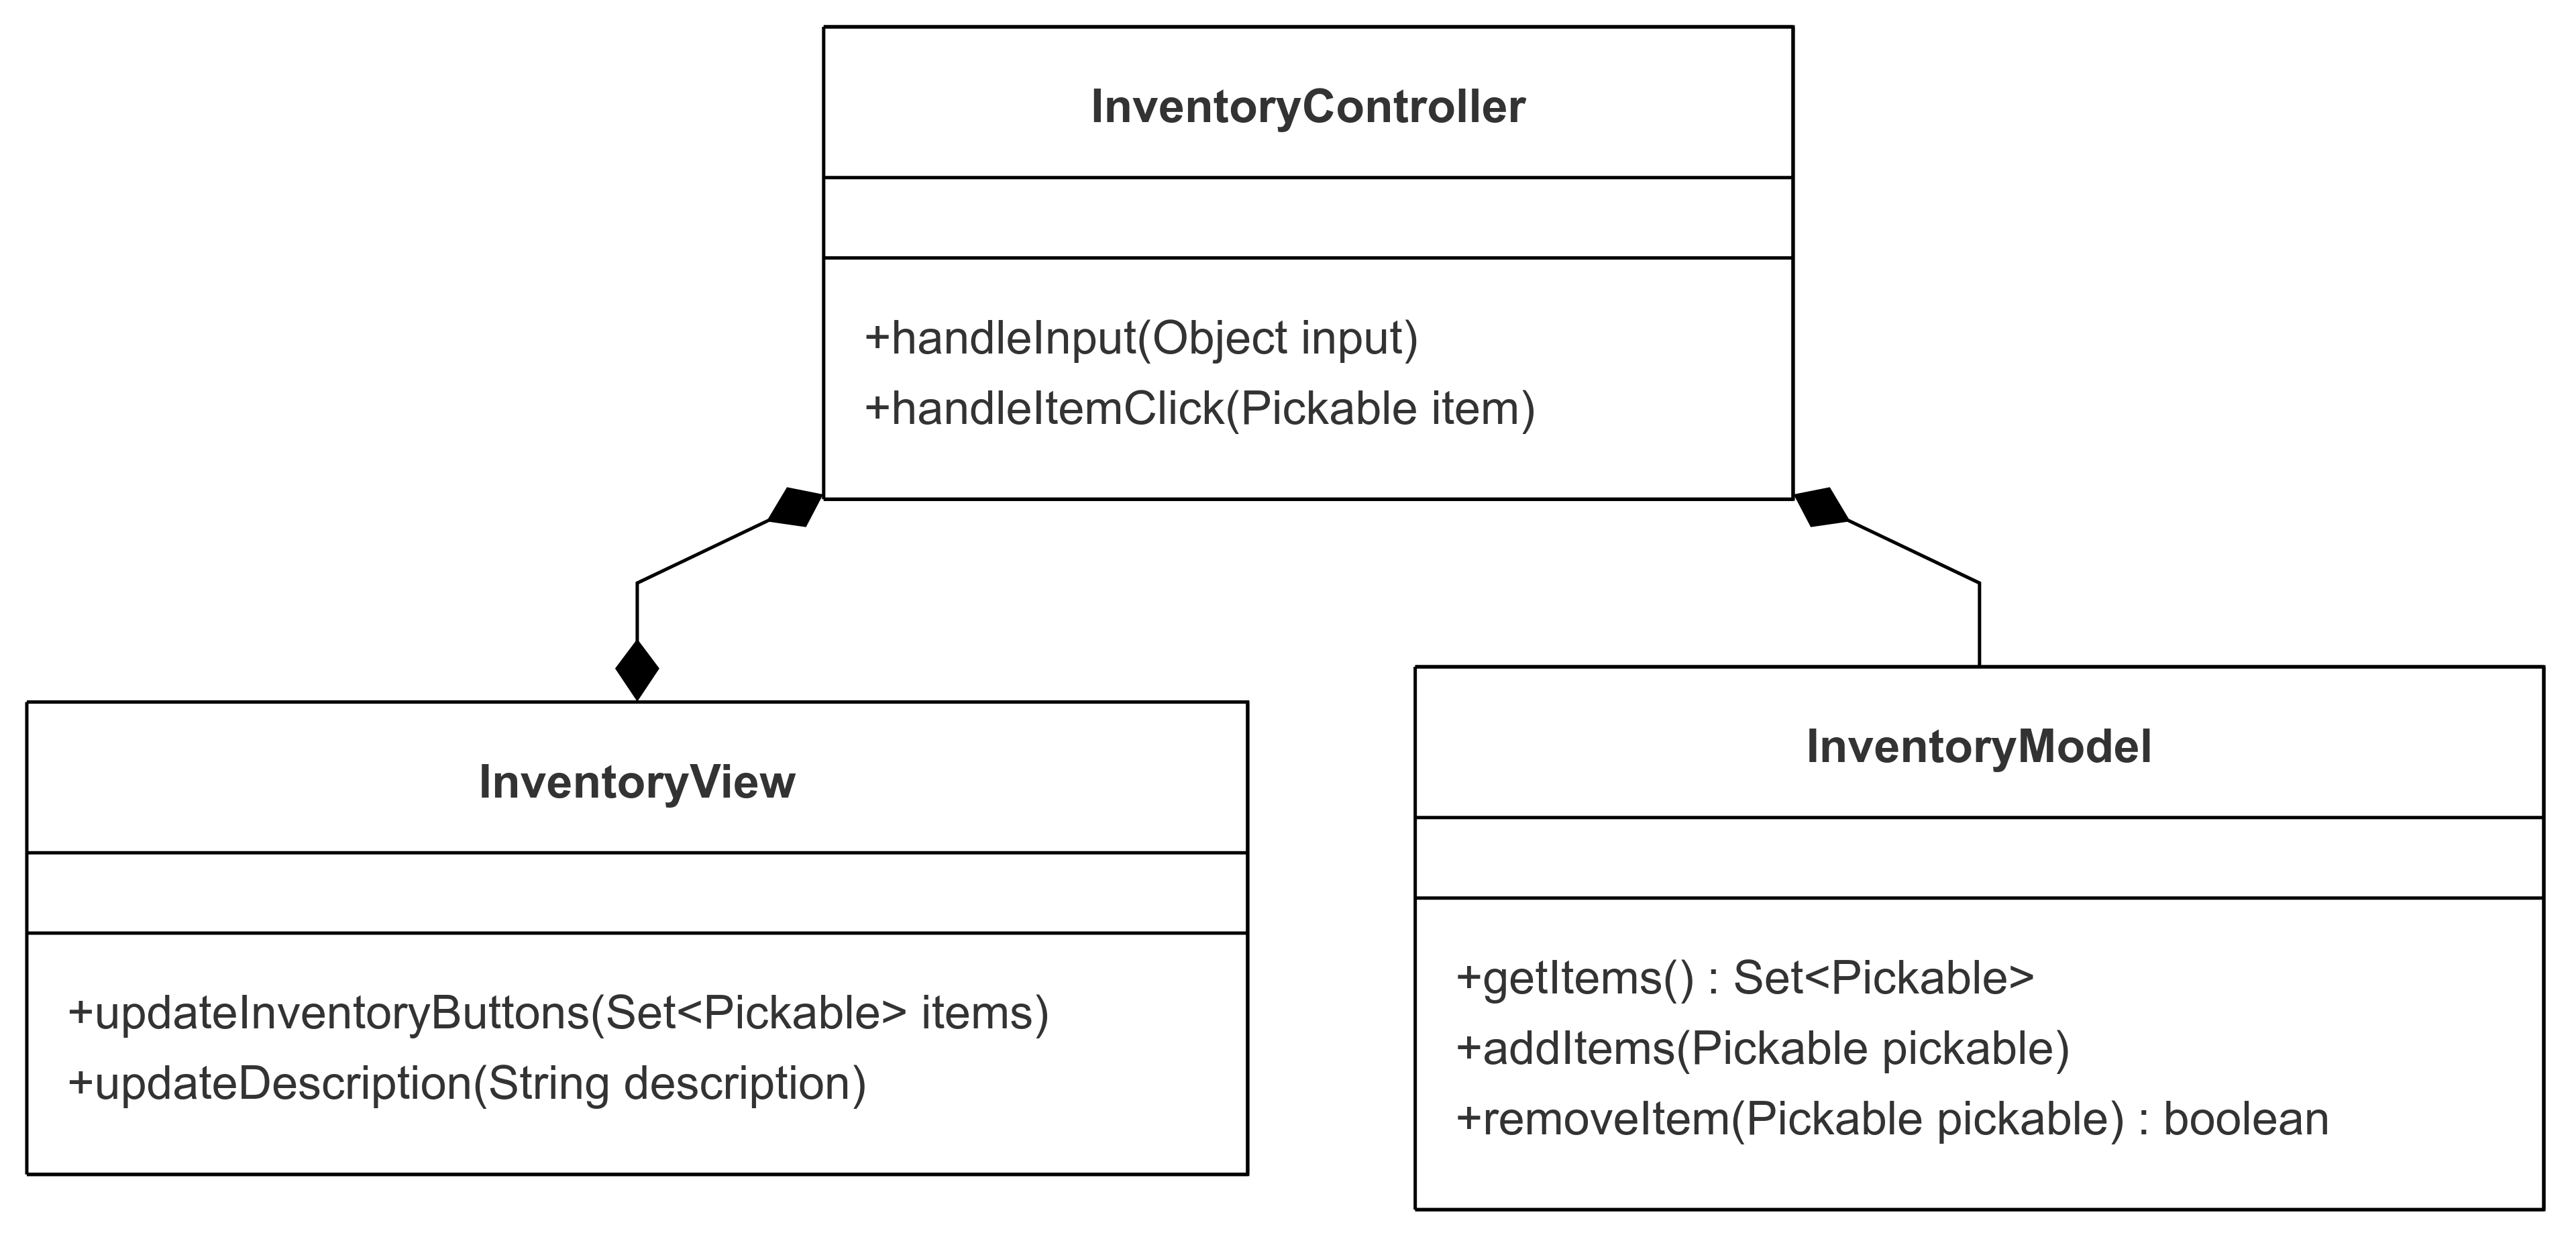
\includegraphics[width=0.8\textwidth]{img/inventory.png}  % Modifica width se serve
    \label{img:gameObject}
\end{figure}
%
\paragraph{Problema}All’interno del gioco sia nell'inventario che nell'enigma del puzzle era necessario che le immagini fornite si adattassero alla dimensione del pulsante (JButton) in cui erano contenute.
%
\paragraph{Soluzione}Per risolvere questo problema, ho creato la classe ImageButton. Questa classe estende JButton e gestisce il ridimensionamento delle immagini in modo che si adattino automaticamente alla dimensione del pulsante. Ho dunque utilizzato questa classe sia nell'inventario che nel puzzle per ridimensionare le immagini direttamente all'interno dei pulsanti.In questo modo, è stato possibile limitare la duplicazione del codice rispettando il principio DRY. Inoltre centralizzando la logica del ridimensionamento delle immagini in una classe specifica, la manutenzione del codice diventa più semplice. 
\begin{figure}[h]  % [h] indica che la figura sarà posizionata il più vicino possibile
    \centering
    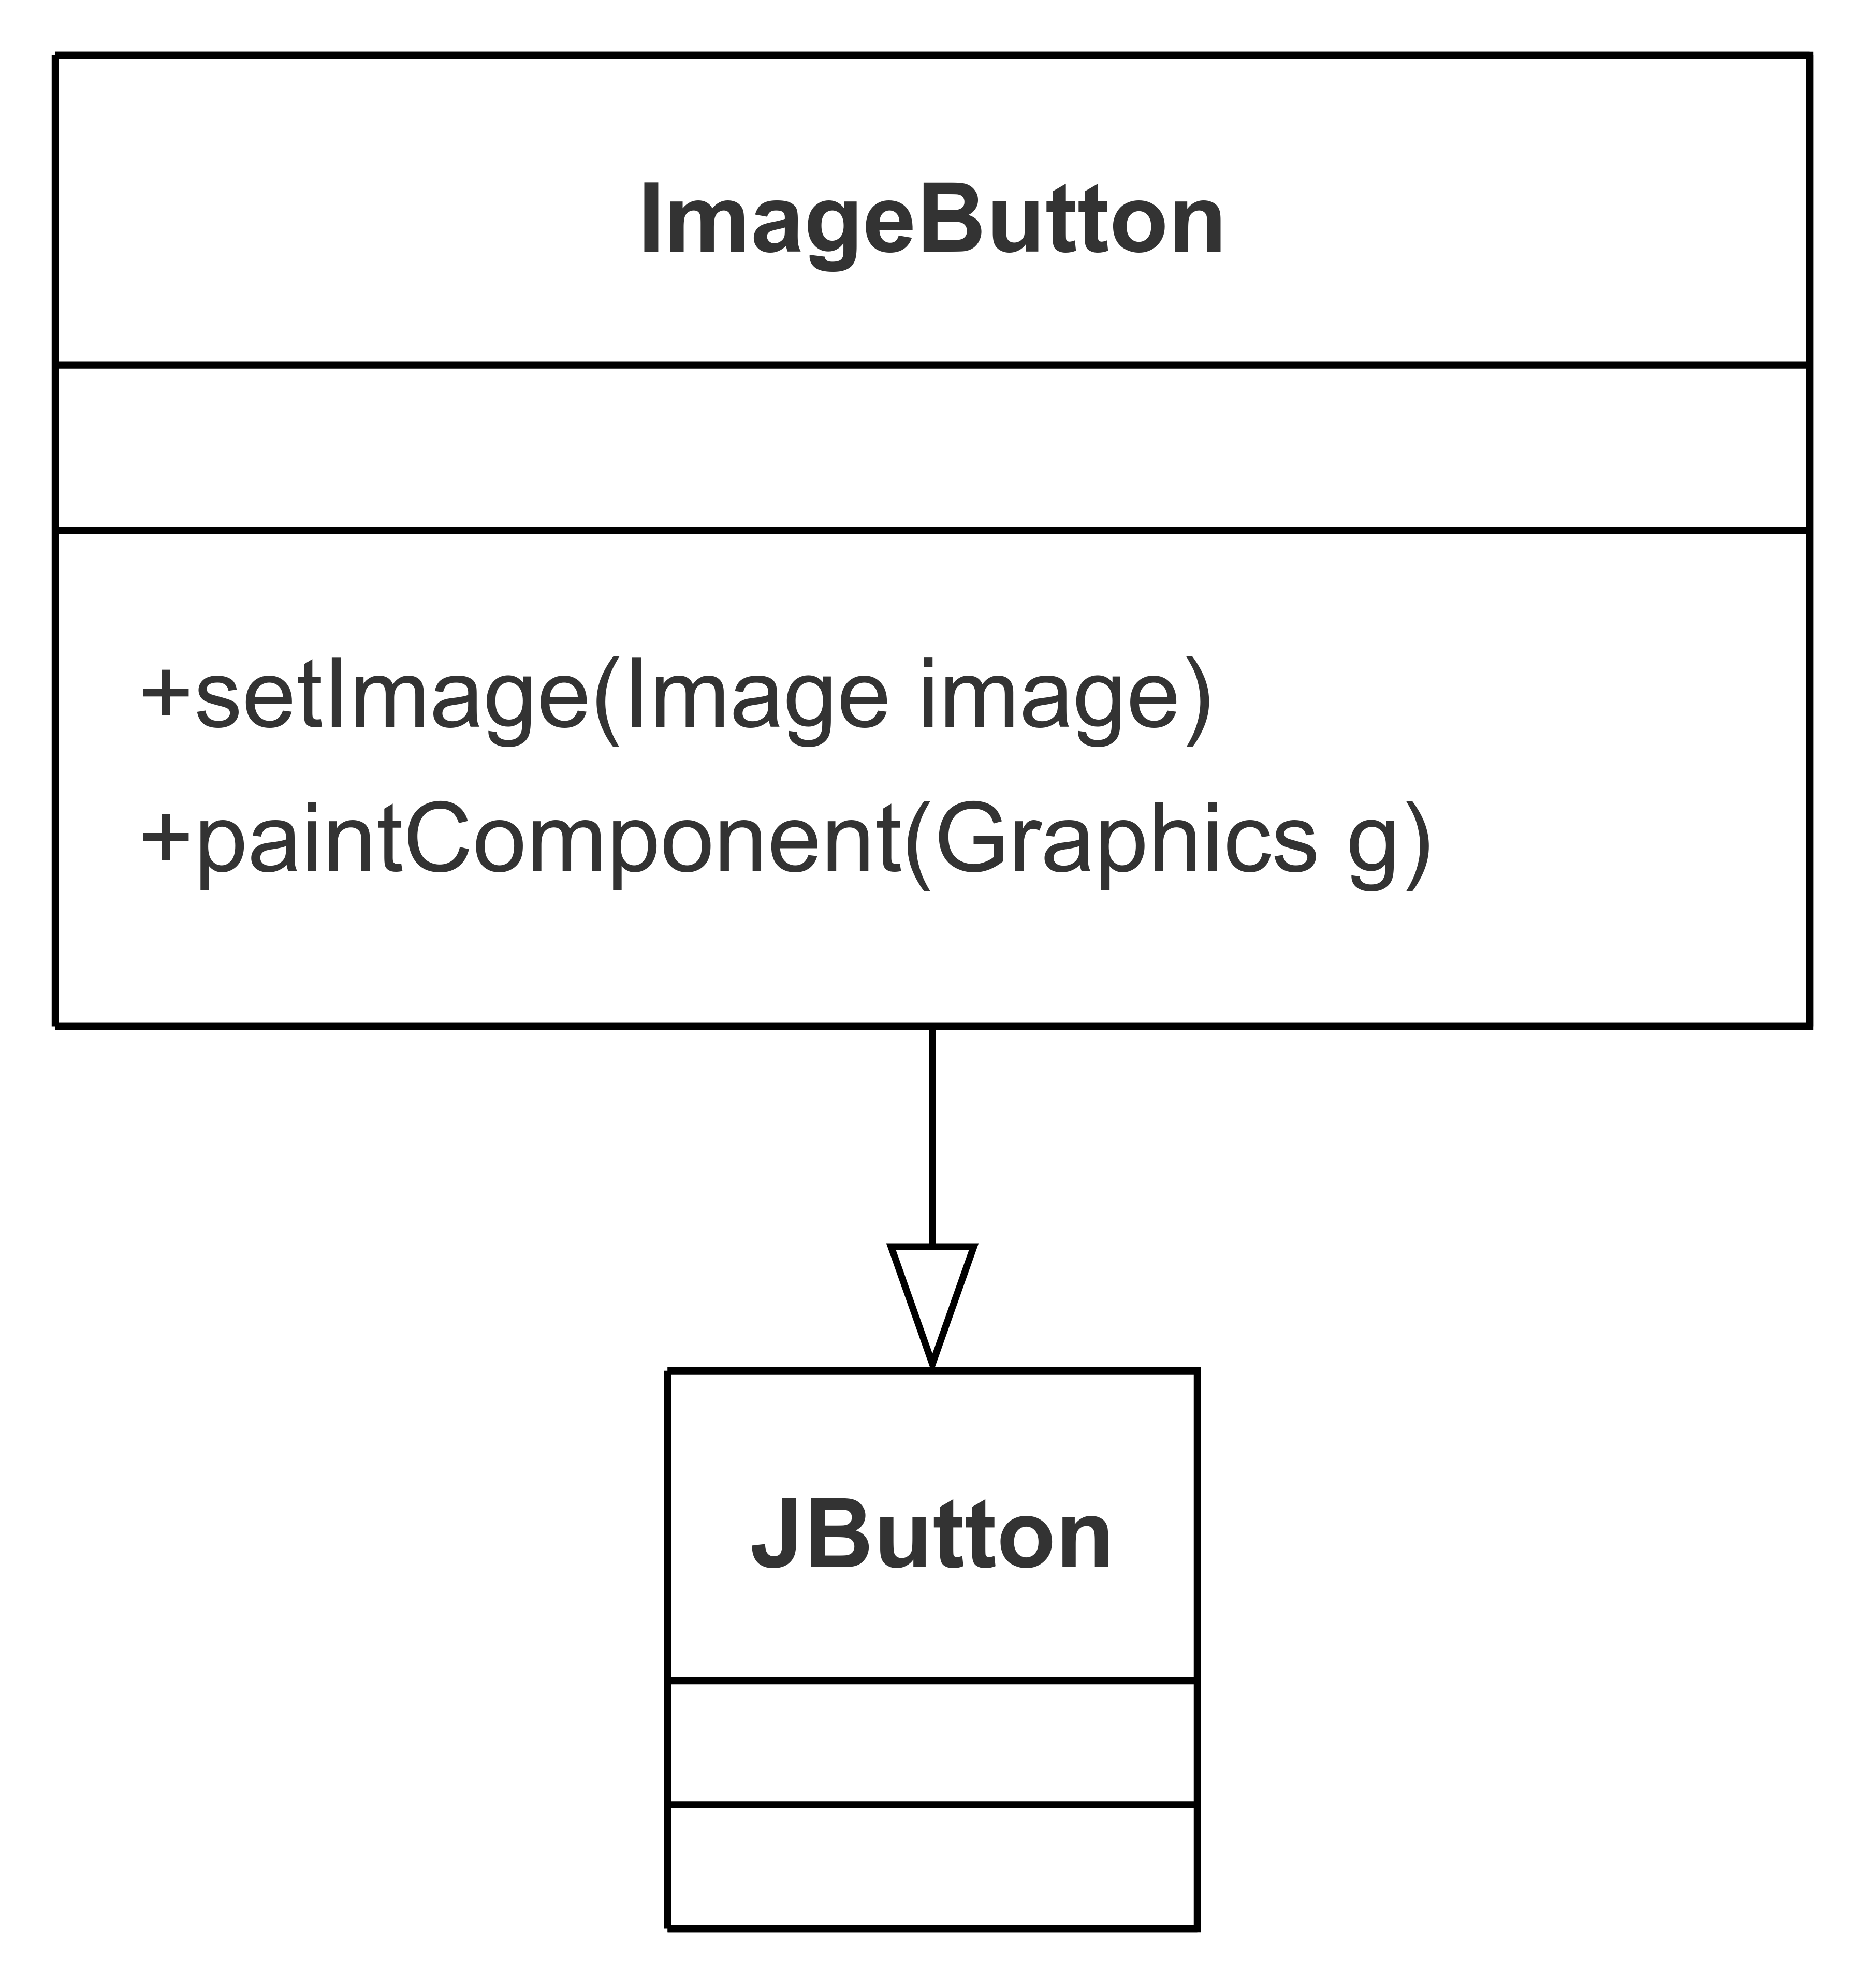
\includegraphics[width=0.8\textwidth]{img/button.png}  % Modifica width se serve
    \label{img:gameObject}
\end{figure}
%
\subsection{Filippo Greppi}
%
%
\paragraph{Problema} Salvataggio e caricamento dello stato di gioco
\paragraph{Soluzione} Il sistema di salvataggio e caricamento utilizza la serializzazione per convertire lo stato del gioco in un formato salvabile su file. Quando il giocatore decide di salvare la partita, il SaveManager prende l'istanza attuale di World che contiene tutte le informazioni sullo stato del gioco, seleziona i dati necessari, e li scrive su file. Quando il giocatore vuole riprendere una partita salvata, il SaveManager legge i dati dal file selezionato ricreando il mondo. Per facilitare la gestione dei salvataggi, la classe Saves permette di ottenere una lista ordinata dei file disponibili, così da poter scegliere facilmente quale caricare.
%
\begin{figure}[h]  % [h] indica che la figura sarà posizionata il più vicino possibile
    \centering
    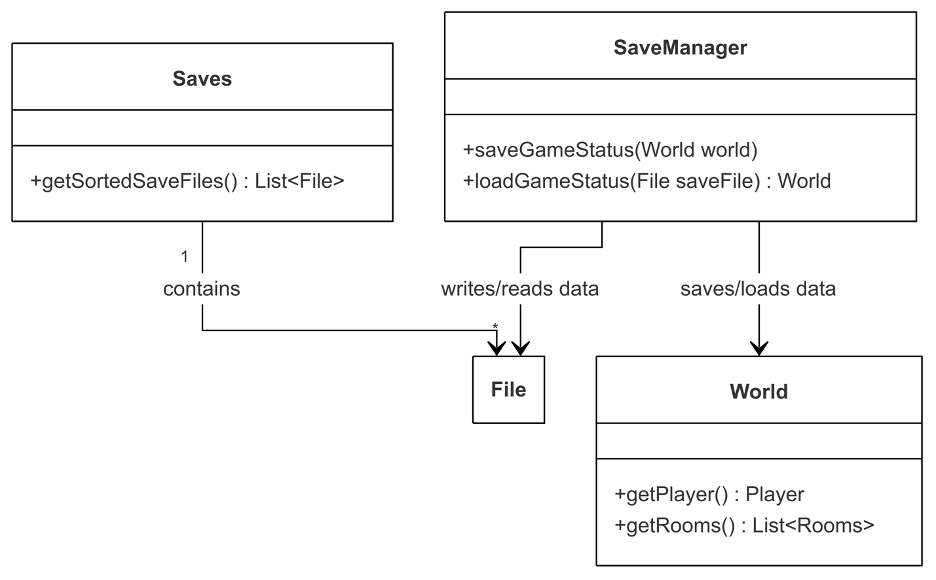
\includegraphics[width=0.8\textwidth]{img/saves.png}  % Modifica width se serve
    \label{img:saves}
\end{figure}
%
\paragraph{Problema} Nel contesto del progetto, il controller principale (MainController) deve gestire dinamicamente diversi componenti del gioco, tra cui menu, enigmi, mondo, e altre sezioni del gioco. Ogni componente del gioco è gestito da un controller separato, ma la creazione e la gestione di questi controller può risultare complessa e propensa a errori se non organizzata correttamente.
\paragraph{Soluzione} La gestione dinamica dei controller è stata implementata utilizzando una combinazione del Factory Pattern e della Controller Map. La classe ControllerFactory funge da punto centrale per la creazione di tutti i controller necessari al gioco. In questo modo, ogni controller viene creato tramite la factory, evitando la ripetizione della logica di creazione in più punti del codice. Se in futuro fosse necessario aggiungere un nuovo controller basterebbe aggiungerlo alla factory. Per facilitare la gestione dei controller durante l’esecuzione del gioco, ho utilizzato una Controller Map, una mappa che tiene traccia di tutti i controller attivi. Ogni controller è associato a un nome univoco, che permette di recuperarlo rapidamente quando necessario. L’integrazione tra la ControllerFactory e la ControllerMap è cruciale per il corretto funzionamento del sistema. Quando un controller è richiesto, se non gia presente, la factory lo crea e lo aggiunge alla mappa dei controller.
%
\begin{figure}[h]  % [h] indica che la figura sarà posizionata il più vicino possibile
    \centering
    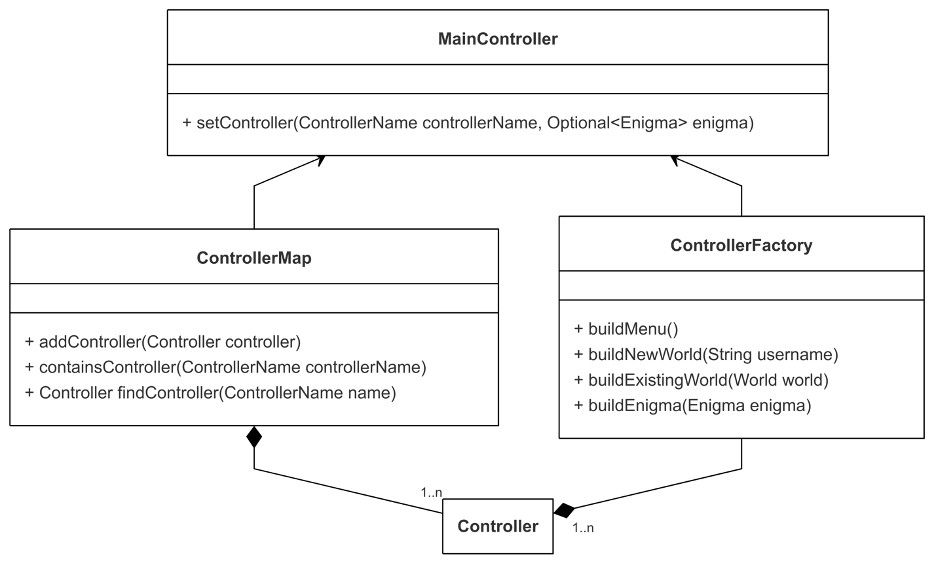
\includegraphics[width=0.8\textwidth]{img/maincontroller.png}  % Modifica width se serve
    \label{img:maincontroller}
\end{figure}

\paragraph{Problema} Identificare i controller diversi all’interno di tutto il sistema.
\paragraph{Soluzione} Per identificare i vari controller all’interno del sistema, ho utilizzato l’enumerazione ControllerName, che rappresenta i nomi dei controller e le loro stringhe corrispondenti. Ogni costante dell’enum è associata a una stringa unica che descrive il controller corrispondente, consentendo una gestione centralizzata e semplificata dei controller.
\begin{figure}[h]  % [h] indica che la figura sarà posizionata il più vicino possibile
    \centering
    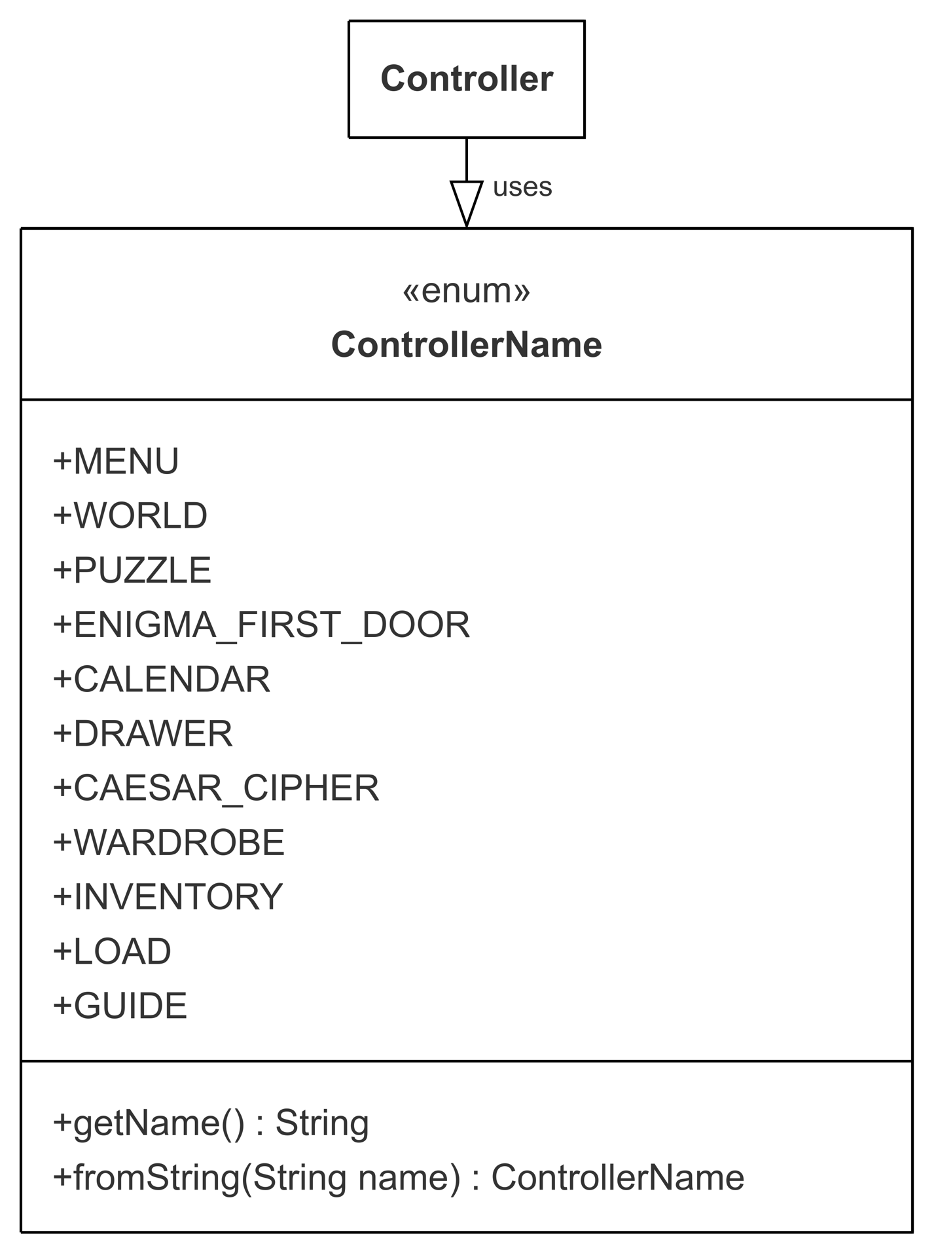
\includegraphics[width=0.8\textwidth]{img/controllerName.png}  % Modifica width se serve
    \label{img:controllerName}
\end{figure}

\paragraph{Problema} Garantire un’esperienza di gioco fluida all’interno del mondo principale
\paragraph{Soluzione} Il WorldController segue un approccio reattivo e dinamico, garantendo una risposta immediata agli input dell’utente senza introdurre ritardi o interruzioni nell’esperienza.
Il controller utilizza un game loop a 60 FPS, regolando il tempo di esecuzione per mantenere costante la fluidità. Il ciclo principale verifica lo stato del gioco, controlla se il giocatore ha vinto, gestisce gli input e aggiorna la visualizzazione. Grazie a questa struttura, il giocatore percepisce un movimento naturale e senza scatti.
Il sistema distingue tra movimenti direzionali (UP, DOWN, LEFT, RIGHT) e azioni specifiche come interagire con oggetti o aprire l’inventario, permettendo al giocatore di esplorare l’ambiente senza interruzioni. Inoltre, se un’azione come INTERACT o INVENTORY viene eseguita, il loop evita input multipli indesiderati.
\begin{figure}[h]  % [h] indica che la figura sarà posizionata il più vicino possibile
    \centering
    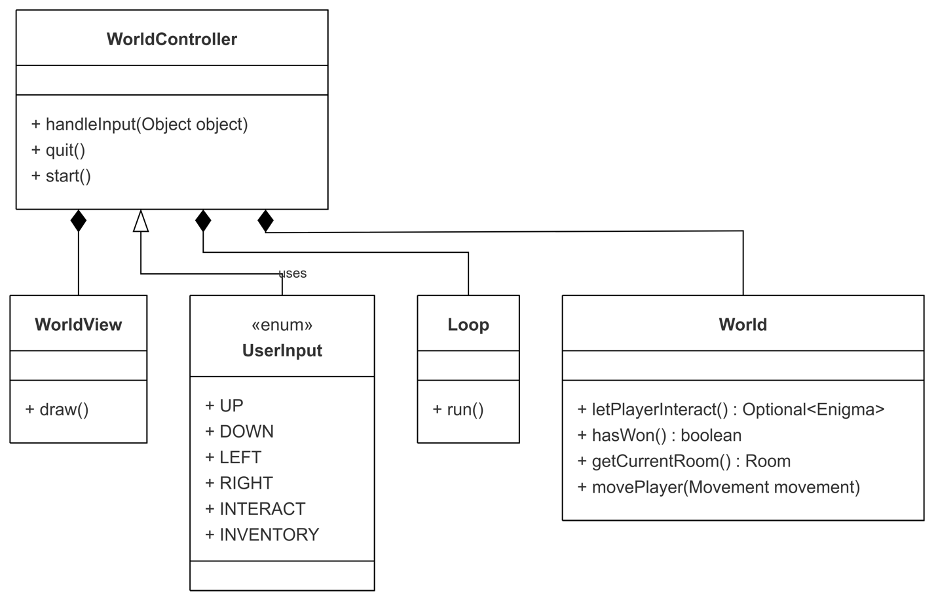
\includegraphics[width=0.8\textwidth]{img/worldController.png}  % Modifica width se serve
    \label{img:controllerName}
\end{figure}
%%
%
\subsection{Ettore Spaccini}
%
\paragraph{Problema} %%descrizione del problema
Creazione delle porte con differenti meccanismi di sblocco.
Nel nostro gioco Mind Escape, le porte possono avere tre stati distinti:
\begin{itemize}
	\item Sempre aperte: permettono il passaggio senza restrizioni.
	\item Bloccate da un enigma: il giocatore deve risolverlo per sbloccarle.
	\item Bloccate da un oggetto (Pickable): il giocatore deve possedere un oggetto specifico nell’inventario per sbloccarle.
\end{itemize}
\paragraph{Soluzione} %% descrizione della soluzione
Utilizzo del Pattern Decorator e del Template Method.
Per garantire flessibilità ed estensibilità, ho adottato due pattern di progettazione:
\begin{itemize}
	\item Pattern Decorator: consente di estendere dinamicamente il comportamento delle porte senza modificare direttamente la classe base.
	\item Pattern Template Method: garantisce che il comportamento delle porte bloccate venga gestito in modo strutturato nelle sottoclassi, evitando duplicazioni di codice.
\end{itemize}
Classi:
\begin{itemize}
	\item Creazione della Porta Base: la classe BaseDoor rappresenta una porta semplice, sempre aperta. Implementa il metodo onAction(Player player), che permette al giocatore di raggiungere la stanza di destinazione.
	\item Decorazione con Enigma: DoorLockedWithEnigma estende AbstractDoorDecorator e richiede la risoluzione di un enigma per lo sblocco.
	\item Decorazione con Pickable: La classe DoorLockedWithPickable segue lo stesso principio, ma invece di un enigma controlla se il giocatore possiede un oggetto con un ID specifico.
\end{itemize}
La logica di sblocco viene gestita attraverso il Template Method isUnlocked() in AbstractDoorDecorator, il quale viene sovrascritto nelle classi derivate per specificare il comportamento di sblocco. 
Questa implementazione permette di aggiungere nuovi tipi di blocco senza modificare la classe DoorImpl, garantendo un design scalabile, mantenibile e seguendo il principio Open-Closed della programmazione a oggetti.
\begin{figure}[h]
    \centering
    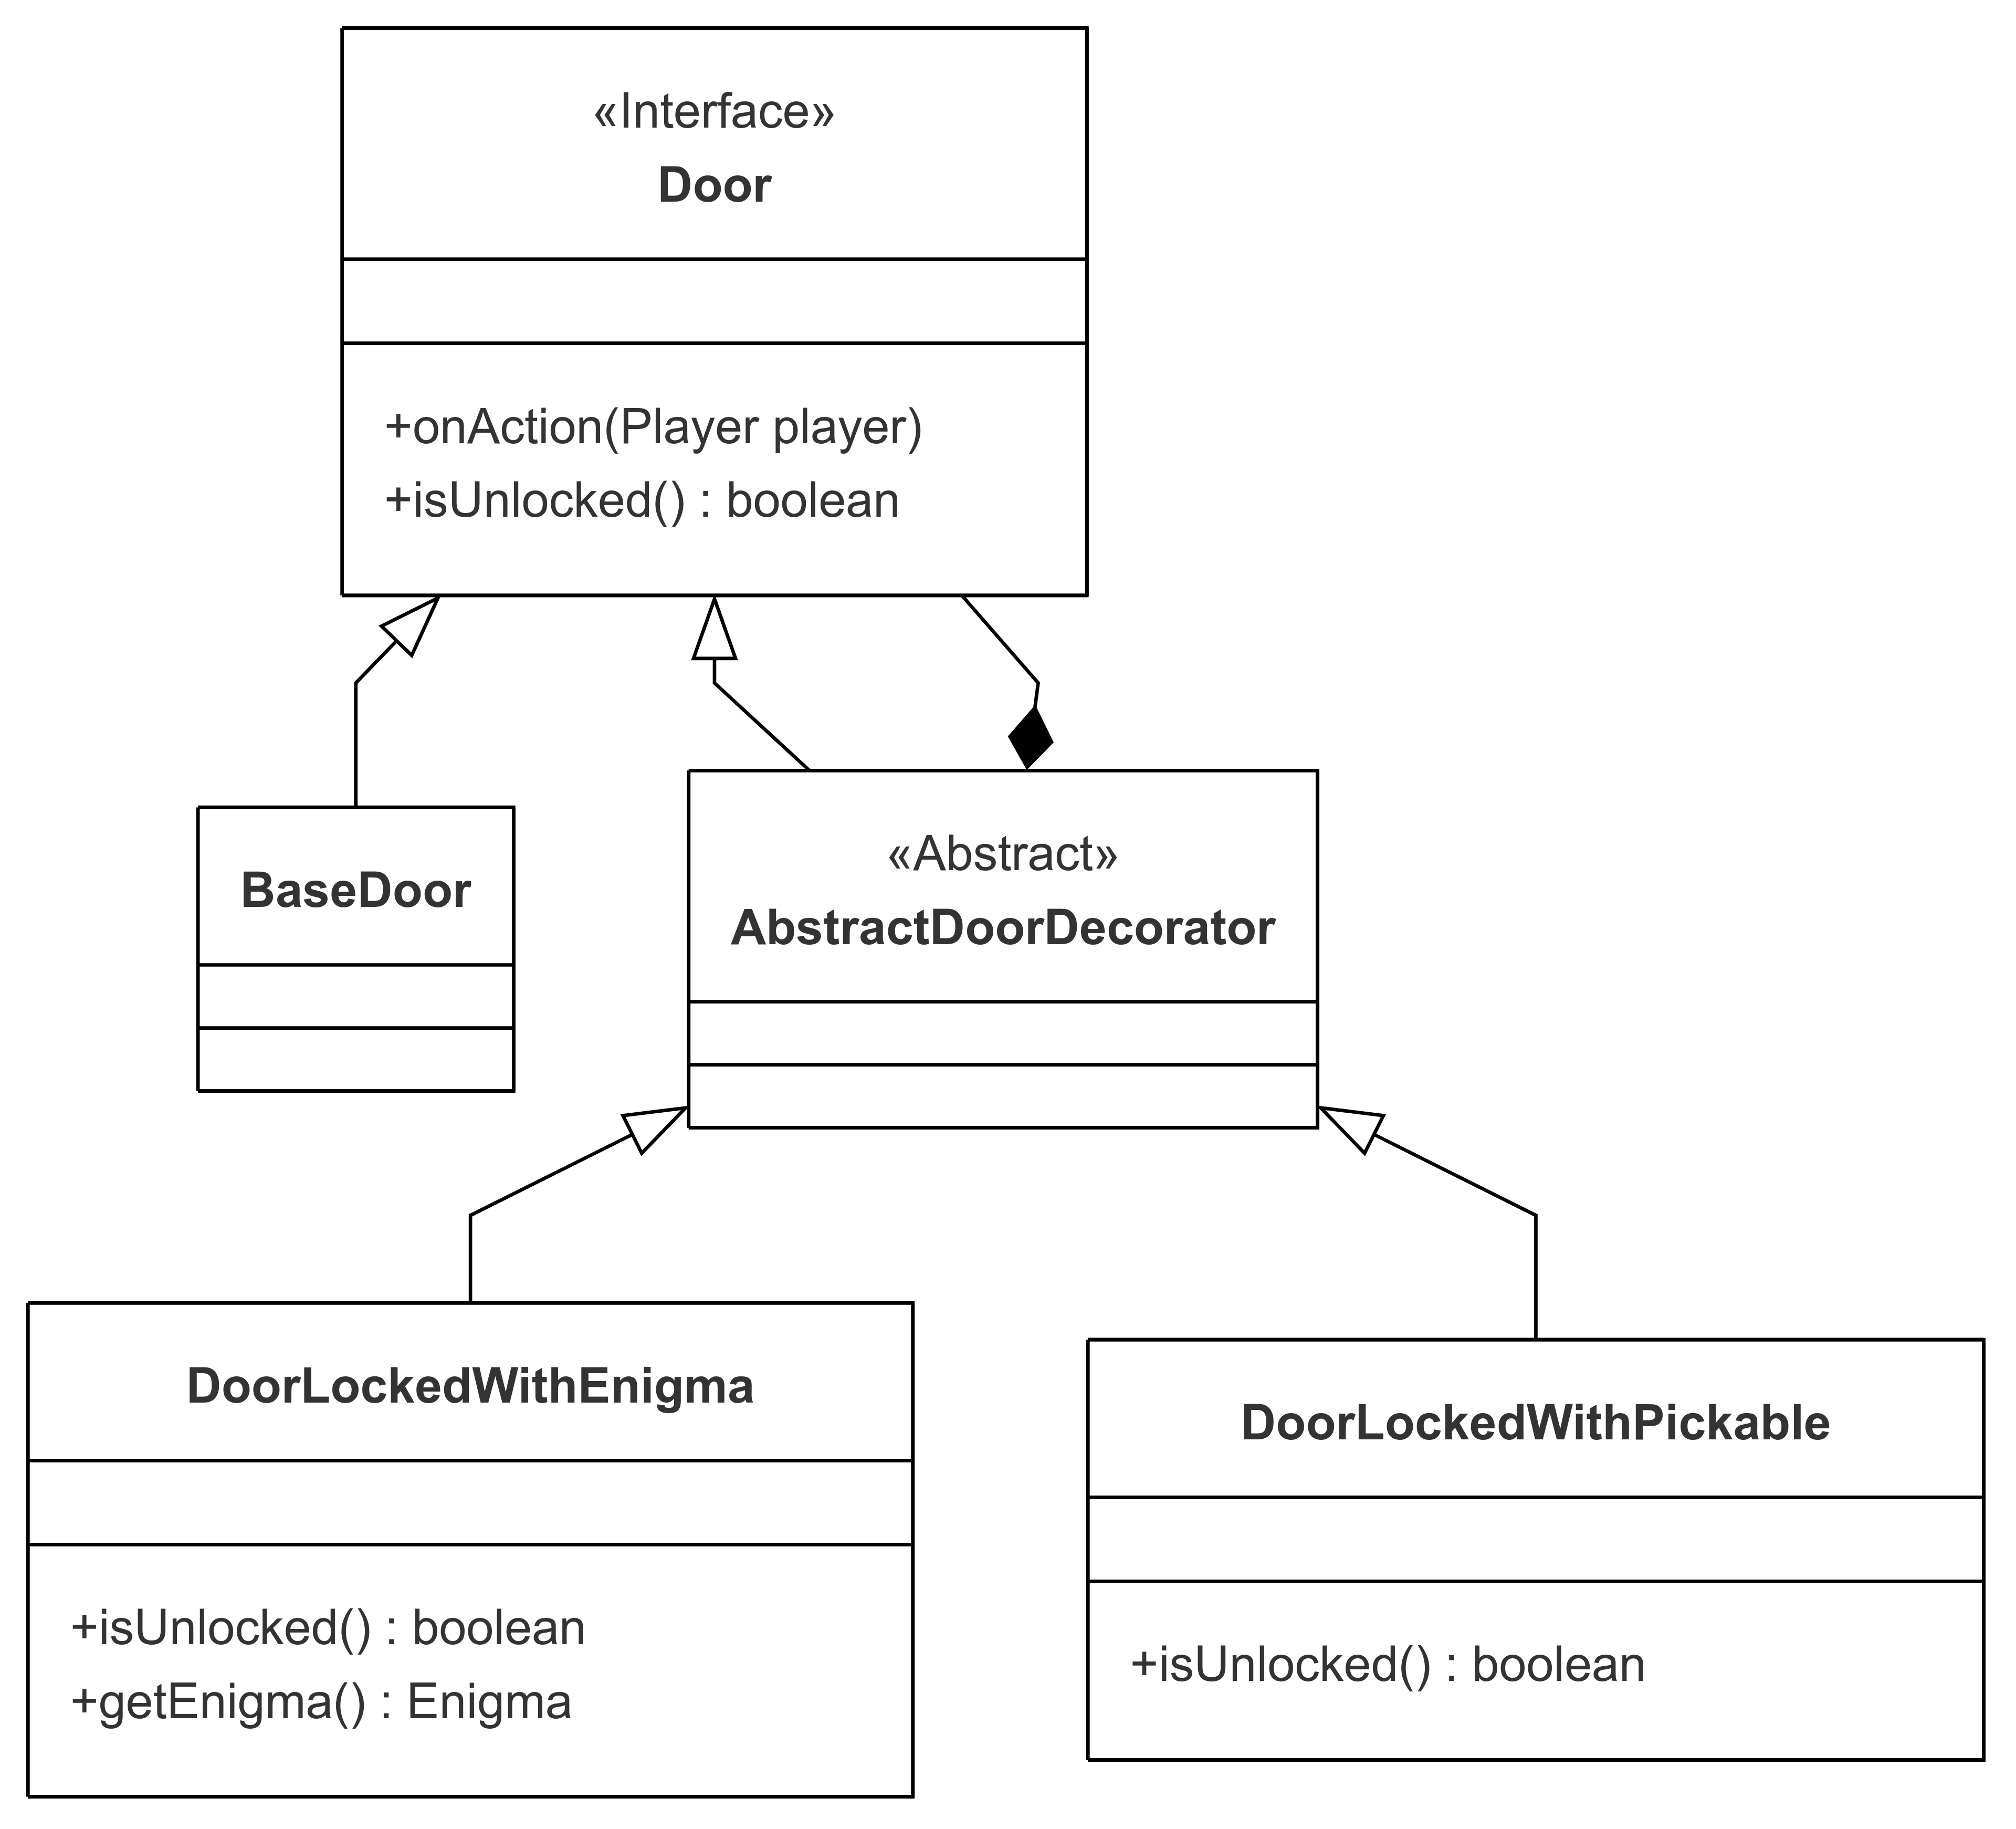
\includegraphics[width=0.8\textwidth]{img/doors.png}
    \label{img:doors}
\end{figure}
\paragraph{Problema} %%descrizione del problema
Creazione degli Oggetti Interagibili (Interactable).
Nel gioco Mind Escape, il personaggio può interagire con diversi tipi di oggetti, ognuno con comportamenti specifici:
\begin{itemize}
	\item Pickable: oggetti raccolti nell'inventario.
	\item Simple Door: porte sempre accessibili senza restrizioni.
	\item DoorLockedWithEnigma: porte sbloccate solo dopo aver risolto un enigma.
	\item DoorLockedWithPickable: porte sbloccate se il giocatore possiede un oggetto specifico.
	\item UnpickableWithEnigma: oggetti non raccoglibili che attivano un enigma.
	\item LockedUnpickable: oggetti non raccoglibili che si sbloccano con un oggetto presente nell'inventario.
	\item Unpickable: oggetti non raccoglibili che, se interagiti, possono rilasciare un oggetto raccoglibile.
\end{itemize}
La gestione separata di questi oggetti avrebbe reso il codice rigido, con molte classi duplicate e difficili da estendere.
\paragraph{Soluzione} %% descrizione della soluzione
Implementazione di una Factory per gli oggetti interagibili.
Per evitare ripetizioni e rendere il codice più modulare, ho utilizzato il Factory Pattern, centralizzando la creazione di tutti gli oggetti interagibili (Interactable). La InteractableFactory fornisce metodi per creare ogni tipo di oggetto interagibile, accettando solo gli attributi essenziali per costruire ciascun oggetto senza duplicare la logica.
Il gioco può così facilmente supportare nuovi oggetti interagibili senza modifiche invasive al codice.
Grazie a questo design, il sistema è più scalabile, chiaro e manutenibile, garantendo una gestione efficiente di tutti gli oggetti con cui il giocatore può interagire.
\begin{figure}[h]
    \centering
    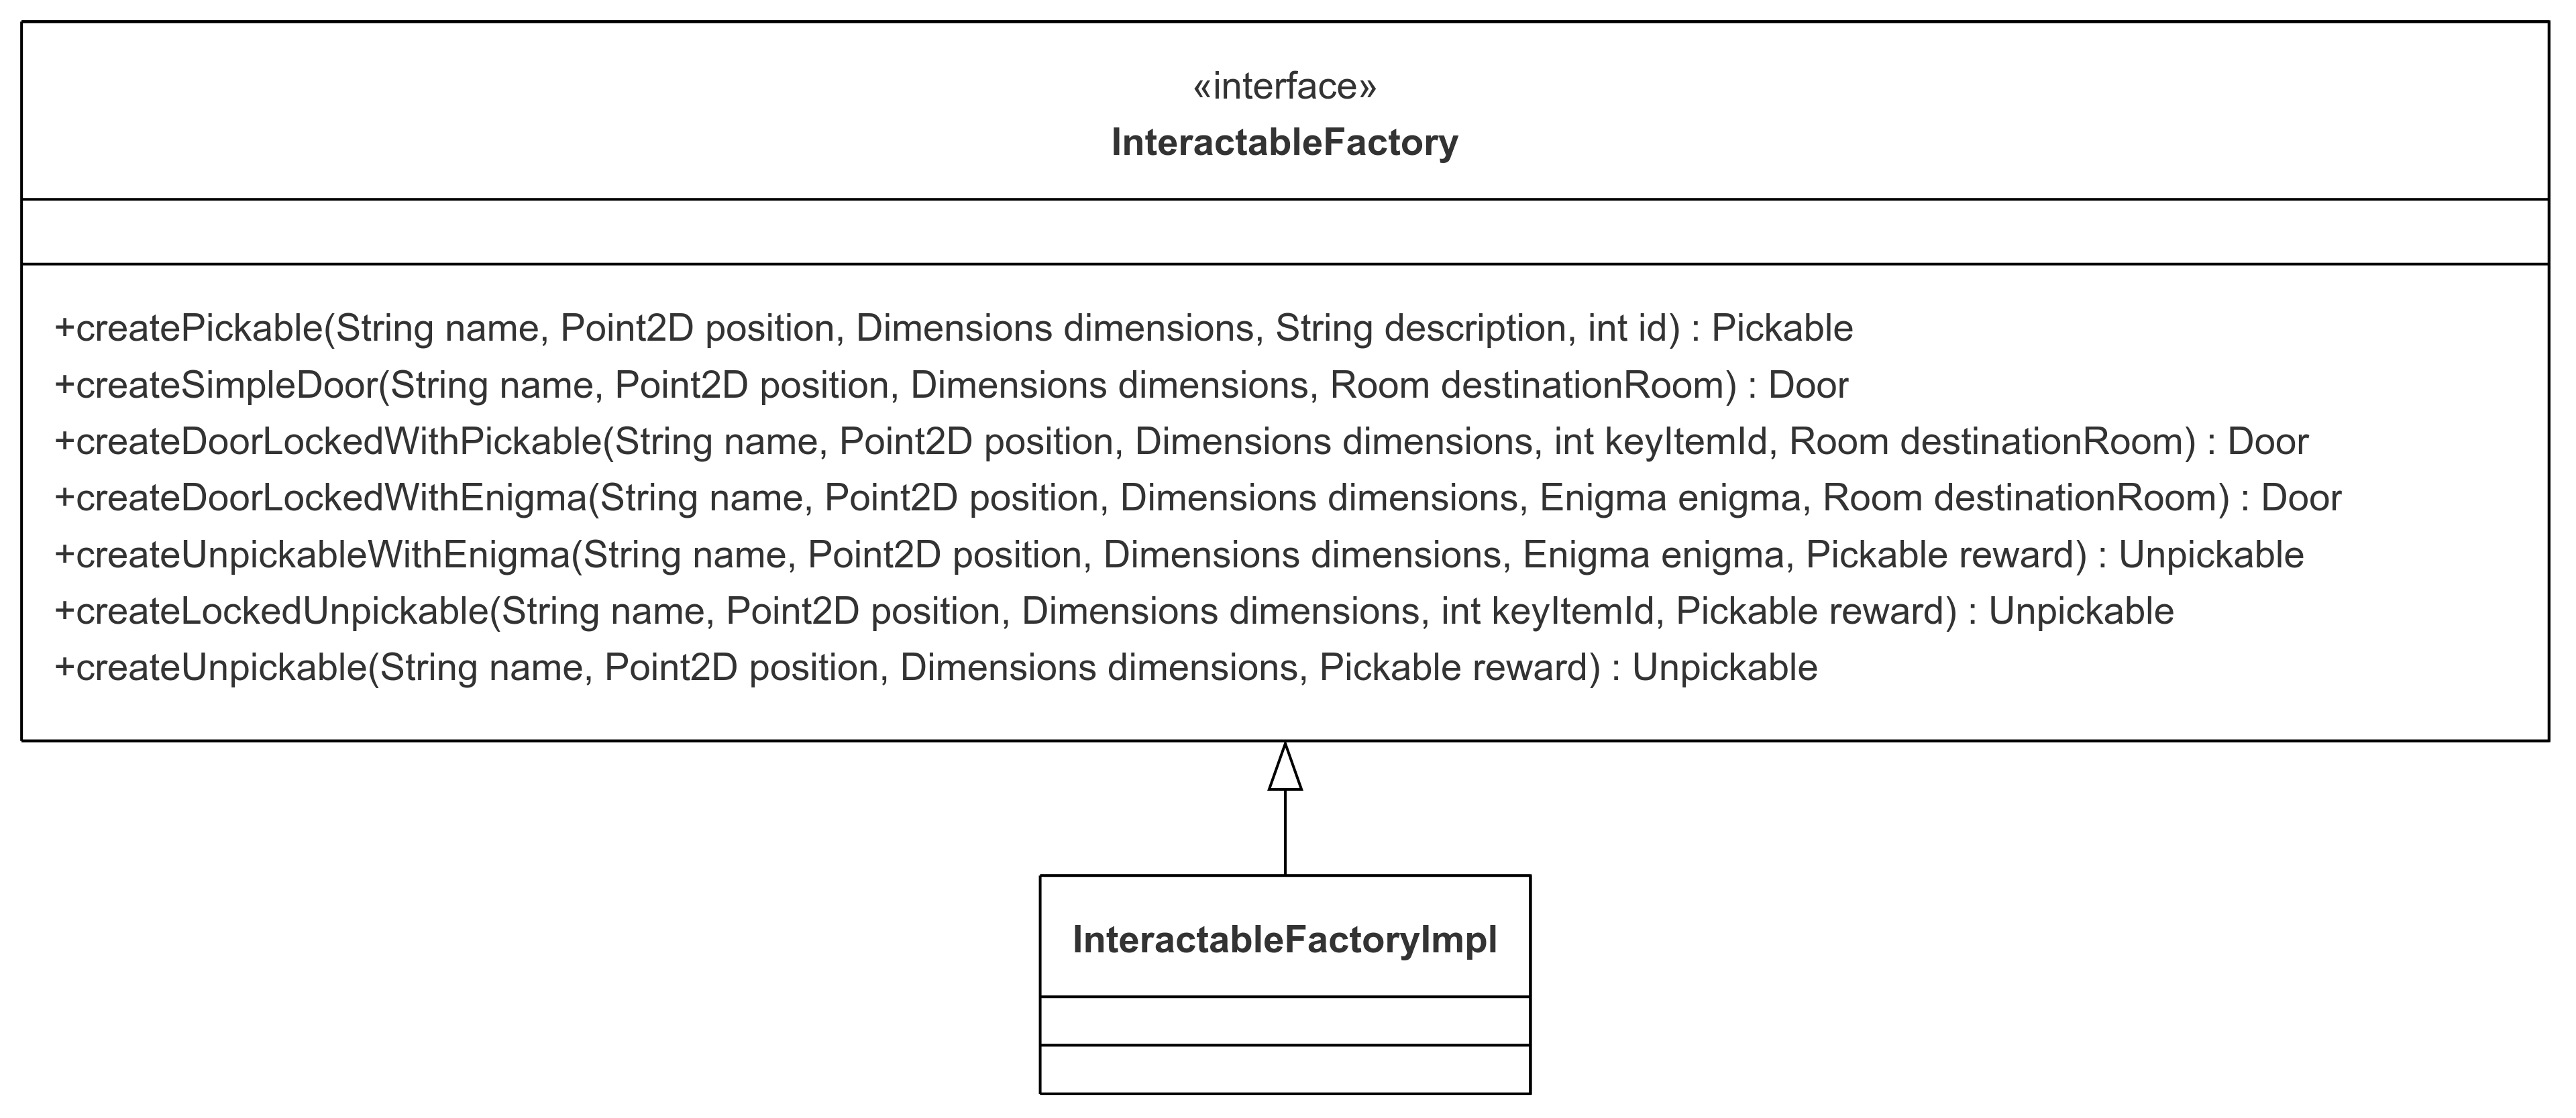
\includegraphics[width=0.8\textwidth]{img/interactableFactory.png}
    \label{img:interactableFactory}
\end{figure}
\paragraph{Problema} %%descrizione del problema
Nel gioco Mind Escape, gli enigmi rappresentano un aspetto fondamentale della progressione. Tuttavia, gestire ogni enigma con una logica monolitica avrebbe reso il codice difficile da mantenere e scalare. Il problema principale era separare la logica di ogni enigma dalla sua interfaccia grafica e dal controllo dell’interazione con l’utente.
\paragraph{Soluzione} %% descrizione della soluzione
Implementazione del Pattern MVC.
Per gestire gli enigmi in modo modulare e scalabile, ho utilizzato il pattern Model-View-Controller (MVC). Ogni enigma è trattato come un'istanza indipendente di MVC, con tre componenti chiave:
\begin{itemize}
	\item Model (CaesarCipherModel, EnigmaPasswordModel)
		\begin{itemize}
			\item Contiene la logica dell’enigma (es. cifratura del testo nel caso del Caesar Cipher).
			\item Memorizza lo stato dell’enigma (risolto o meno).
			\item Implementa metodi per verificare la soluzione.
		\end{itemize}
	\item View (CaesarCipherViewImpl, EnigmaPasswordViewImpl)
		\begin{itemize}
			\item Gestisce l’interfaccia grafica, visualizzando l’enigma e i risultati dell’interazione.
			\item Riceve input dall’utente (es. shift per la cifratura, password per l’enigma testuale).
			\item Mostra il feedback all’utente.
		\end{itemize}
	\item Controller (CaesarCipherControllerImpl, EnigmaPasswordControllerImpl)
		\begin{itemize}
			\item Interpreta l’input dell’utente e aggiorna il Model di conseguenza.
			\item Chiede alla View di aggiornare la UI in base ai cambiamenti nel Model.
			\item Comunica con il MainController per gestire il flusso del gioco e notificarlo a seguito della terminazione di un enigma, reimpostando come controller corrente quello del World.
		\end{itemize}
\end{itemize}
Vantaggi:
\begin{itemize}
	\item Separazione delle responsabilità: ogni componente è responsabile di un solo aspetto. 
	\item Manutenibilità migliorata: è possibile aggiornare la logica di un enigma senza toccare la UI o il controller.
	\item Maggiore modularità: gli enigmi possono essere facilmente riutilizzati o modificati per adattarsi a nuove esigenze.
\end{itemize}
\begin{figure}[h]
    \centering
    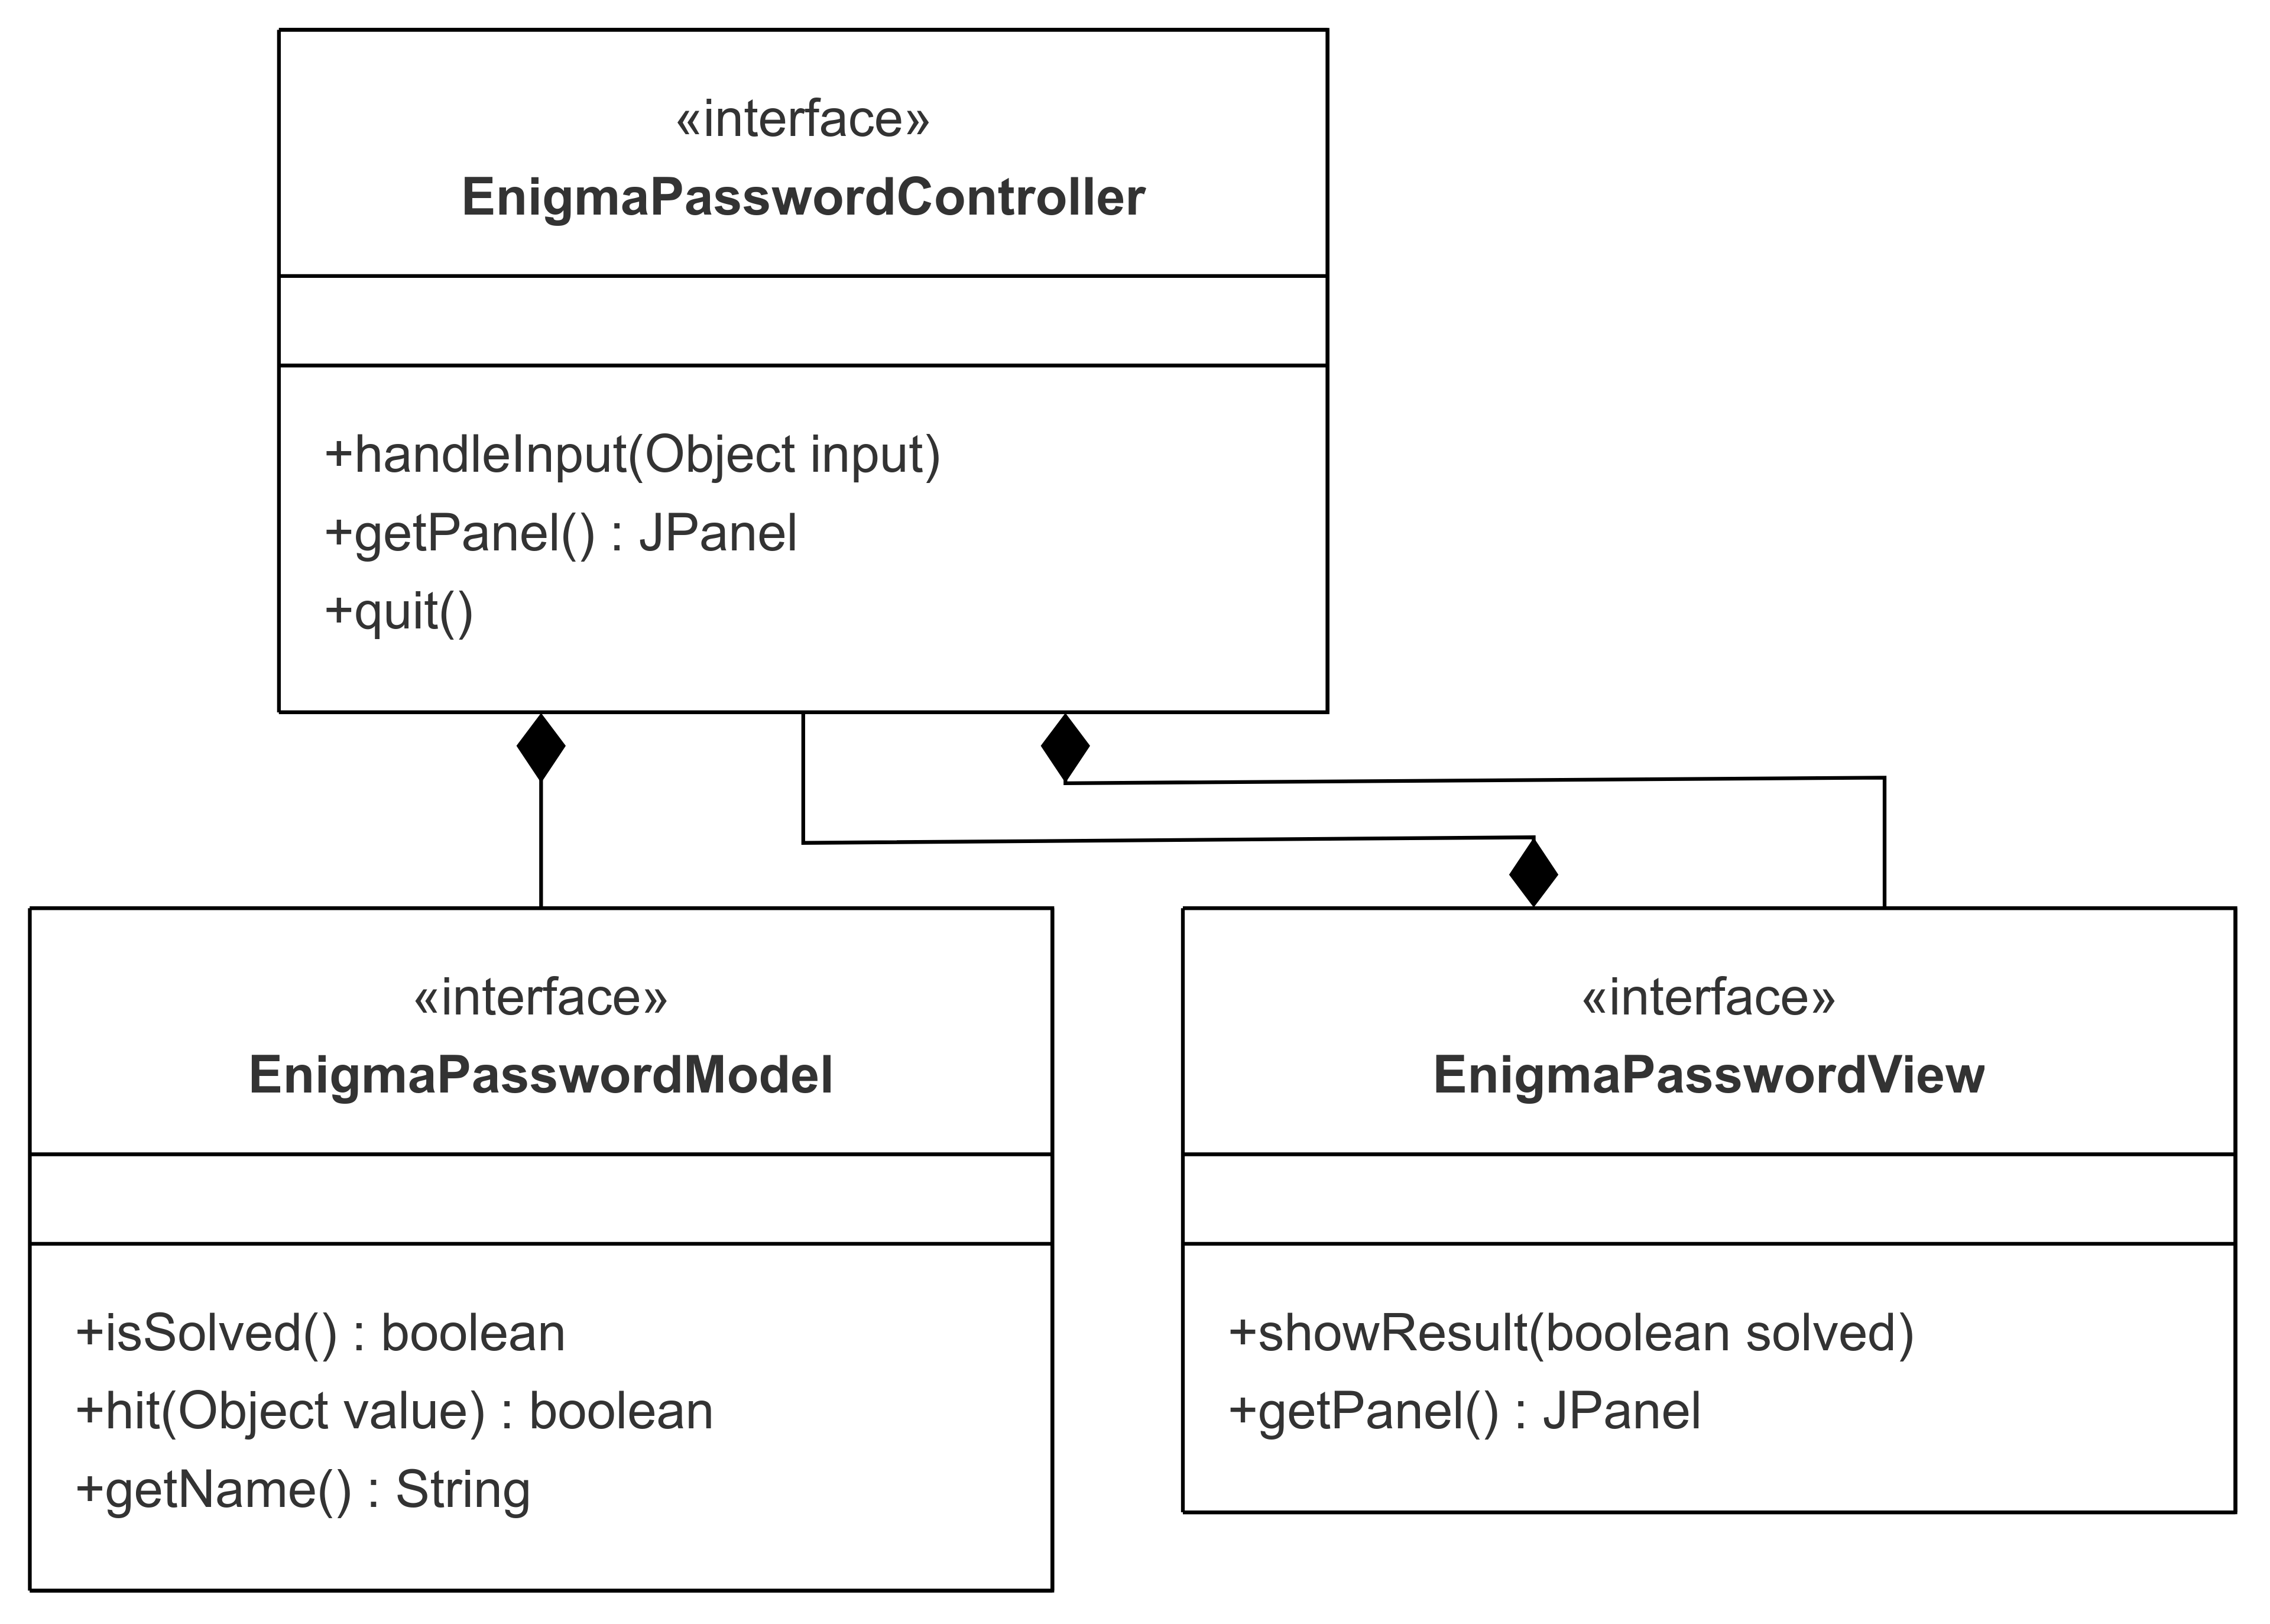
\includegraphics[width=0.8\textwidth]{img/enigmaPassword.png}
    \label{img:enigmaPassword}
\end{figure}
\begin{figure}[h]
    \centering
    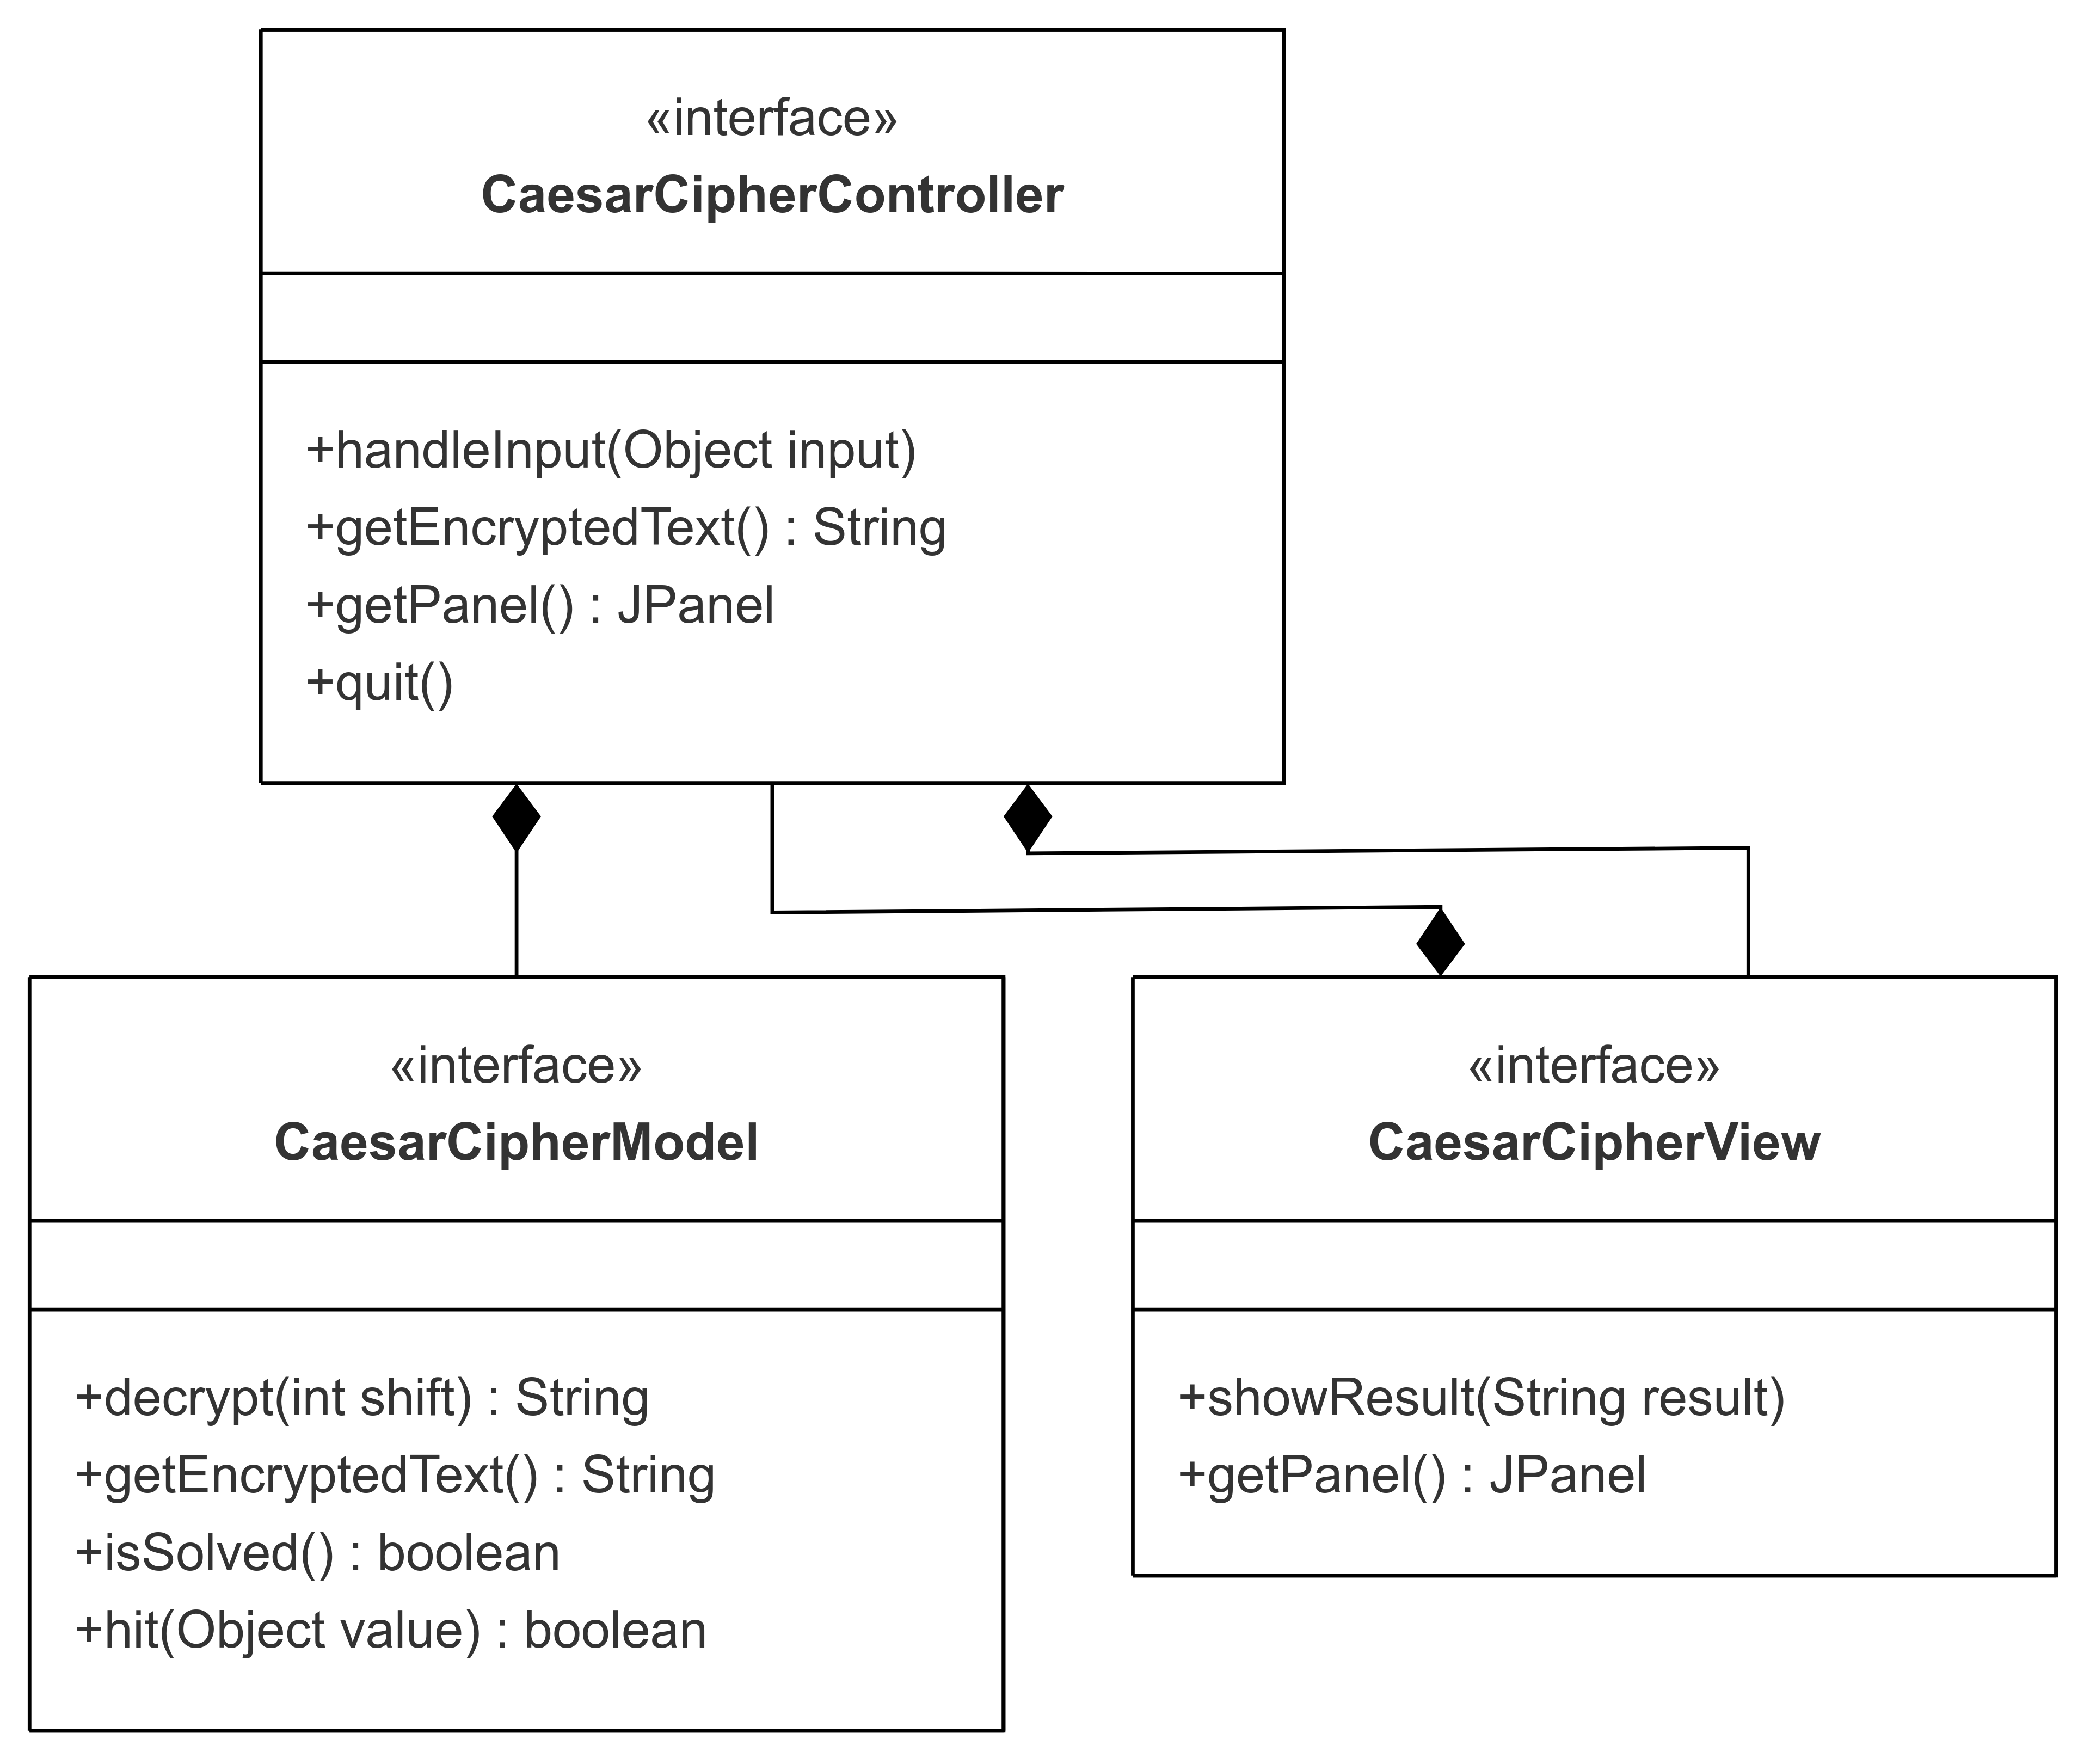
\includegraphics[width=0.8\textwidth]{img/caesarCipher.png}
    \label{img:caesarCipher}
\end{figure}
%
\subsection{Marcello Spagnoli}
%
\paragraph{Problema} %%descrizione del problema
\paragraph{Soluzione} %% descrizione della soluzione
%


\chapter{Sviluppo}
\section{Testing automatizzato}

\begin{itemize}
	\item 
	% inserire quali test sono stati fatti e come sono stati fatti

\end{itemize}


\section{Note di sviluppo}

% qui vanno inseriti i permalink

\chapter{Commenti finali}


\section{Autovalutazione e lavori futuri}

%
Ciascuno dovrà autovalutare il proprio lavoro, elencando i punti di forza e di debolezza in quanto prodotto.
Si dovrà anche cercare di descrivere \emph{in modo quanto più obiettivo possibile} il proprio ruolo all'interno del gruppo.
Si ricorda, a tal proposito, che ciascuno studente è responsabile solo della propria sezione: non è un problema se ci sono opinioni contrastanti, a patto che rispecchino effettivamente l'opinione di chi le scrive.
Nel caso in cui si pensasse di portare avanti il progetto, ad esempio perché effettivamente impiegato, o perché sufficientemente ben riuscito da poter esser usato come dimostrazione di esser capaci progettisti, si descriva brevemente verso che direzione portarlo.

\section{Difficoltà incontrate e commenti per i docenti}

Questa sezione, \textbf{opzionale}, può essere utilizzata per segnalare ai docenti eventuali problemi o difficoltà incontrate nel corso o nello svolgimento del progetto, può essere vista come una seconda possibilità di valutare il corso (dopo quella offerta dalle rilevazioni della didattica) avendo anche conoscenza delle modalità e delle difficoltà collegate all'esame, cosa impossibile da fare usando le valutazioni in aula per ovvie ragioni.
%
È possibile che alcuni dei commenti forniti vengano utilizzati per migliorare il corso in futuro: sebbene non andrà a vostro beneficio, potreste fare un favore ai vostri futuri colleghi.
%
Ovviamente \textit{il contenuto della sezione non impatterà il voto finale}.

\appendix
\chapter{Guida utente}

I comandi di gioco sono i seguenti:
\begin{itemize}
	\item \textbf{W, A, S, D}: per muovere il personaggio
	\item \textbf{E}: per interagire con gli oggetti
	\item \textbf{I}: per aprire l'inventario
\end{itemize}

\chapter{Guida soluzione}
%
\section{Stanza 1 - Camera da Letto}
\begin{itemize}
	\item Interagendo con letto si raccoglie un biglietto 
	\item Interagendo con il tavolo si apre un puzzle 
	\item la porta si sblocca inserendo la password “Sergio Mattarella”
\end{itemize}
%
\section{Stanza 2 - Mensa}
\begin{itemize}
	\item Raccogliere il biglietto sul tavolo 
	\item Guardare il calendario (vicino alla porta di entrata) come suggerisce il biglietto 
	\item Interagire con la cassettiera vicino al calendario (Password: “12-13”) 
	\item Interagire di nuovo con la cassettiera per prendere la chiave (che sblocca una delle due porte) 
	\item Raccogliere la chiave inglese  
	\item Provare a sbloccare una delle 2 porte
\end{itemize}
%
\section{Stanza 3 - Ufficio}
\begin{itemize}
	\item Raccogliere la torcia 
	\item Interagire col computer (Shift: “3”) 
	\item Tornare alla mensa 
	\item Tentare di sbloccare la porta rimasta 
\end{itemize}
%
\section{Stanza 4 - Archivio}
\begin{itemize}
	\item Aprire la cassa raccogliendo il martello
	\item Andare nell’ armadio in mezzo alla stanza e inserire la password del cifrario: “oblivion” 
	\item Interagire di nuovo con l’armadio per prendere il biglietto al suo interno (che sblocca l’ultima porta) 
\end{itemize}
%
\section{Stanza 5 - Finale}
\begin{itemize}
	\item Interagire con lo specchio
\end{itemize}

\appendix
\chapter{Esercitazioni di laboratorio}

 
\subsection{ettore.spaccini@studio.unibo.it}

\begin{itemize}
 \item Laboratorio 09: \url{https://virtuale.unibo.it/mod/forum/discuss.php?d=179154#p248293}
 \item Laboratorio 10: \url{https://virtuale.unibo.it/mod/forum/discuss.php?d=180101#p248884}
\end{itemize}


 % non toccare nulla

\bibliographystyle{alpha}
\bibliography{13-template}

\end{document}
